\documentclass{article}
\usepackage[utf8]{inputenc}
\usepackage[left=2.5cm, top=2.5cm, right=2.5cm, bottom=2.5cm]{geometry}
\usepackage[spanish]{babel}
\usepackage{hyperref}
\usepackage{graphicx}
\usepackage{float}
\usepackage{listings}
\usepackage{xcolor}

\setlength{\parskip}{10pt}
\definecolor{vscdbg}{rgb}{0.80,0.80,0.85}      % Slightly darker Background
\definecolor{vscdstring}{rgb}{0.13,0.55,0.13}  % Strings (green)
\definecolor{vscdcomment}{rgb}{0.46,0.54,0.60} % Comments
\definecolor{vscdkeyword}{rgb}{0.56,0.38,0.68} % Keywords (darker for contrast)
\definecolor{vscdnumber}{rgb}{0.48,0.38,0.26}  % Numbers (darker for contrast)
\definecolor{vscdgray}{rgb}{0.40,0.40,0.40}    % Line numbers
\definecolor{vscdtext}{rgb}{0.30,0.30,0.30}    % Main text (lighter gray)
\lstdefinestyle{mystyle}{
    backgroundcolor=\color{vscdbg},
    basicstyle=\ttfamily\footnotesize\color{vscdtext},
    commentstyle=\color{vscdcomment}\itshape,
    numberstyle=\tiny\color{vscdgray},
    stringstyle=\color{vscdstring},
    breakatwhitespace=false,
    captionpos=b,
    numbers=left,
    showspaces=false,
    showstringspaces=false,
    showtabs=false,
    xleftmargin=50pt,
    xrightmargin=50pt,
    frame=single,
    aboveskip=10pt,
    belowskip=10pt,
    columns=flexible
}

\lstset{style=mystyle}

\definecolor{consolebg}{rgb}{0.95,0.95,0.92}
\definecolor{consoletext}{rgb}{0.20,0.20,0.20}
\definecolor{consoleprompt}{rgb}{0.60,0.60,0.60}
\lstdefinestyle{console}{
    backgroundcolor=\color{consolebg},
    basicstyle=\ttfamily\footnotesize\color{consoletext},
    numberstyle=\tiny\color{consoleprompt},
    commentstyle=\color{consoleprompt}\itshape,
    showstringspaces=false,
    showspaces=false,
    showtabs=false,
    frame=single,
    xleftmargin=30pt,
    xrightmargin=30pt,
    aboveskip=8pt,
    belowskip=8pt,
    columns=flexible,
    numbers=none,
    keywordstyle=\color{consoleprompt},
    moredelim=**[is][\color{consoleprompt}]{@}{@}
}

\linespread{1}
\hypersetup{
    pdftitle={(TA047) Trabajo Práctico 1},
    pdfauthor={Patricio Ibar - 109569},
    pdfsubject={Informe del Trabajo Práctico 1 de la materia Ciencia de Datos TA047},
}
\title{
    
\includegraphics[width=0.5\textwidth]
    {imagenes/Logo-fiuba.png}

    \vspace{1cm}
    \textbf{(TA047) - Ciencia de Datos} \\
    \vspace{1cm}
    \textbf{Trabajo Práctico 1 (2C2025)}
}
\author{Patricio Ibar - Padrón 109569}
\date{11 de septiembre de 2025}

\begin{document}
    
    \maketitle
    \newpage

    \tableofcontents
    \newpage

    \section{Introducción}
En el presente informe se documentan los pasos seguidos para la realización del Trabajo Práctico 1 de la materia Ciencia de Datos (TA047) de la Facultad de Ingeniería de la Universidad de Buenos Aires. El objetivo del trabajo práctico es realizar un análisis exploratorio de conjunto de datos. El análisis incluye la limpieza y preparación de los datos, la realización de consultas y visualizaciones, y la interpretación de los resultados obtenidos. La consigna del trabajo práctico y los datos a analizar pueden encontrarse en el siguiente enlace: \url{https://organizacion-de-datos-7506-argerich.github.io/consigna_tp1_2c2025.html}.

Se trabajó utilizando Python y la librería pandas para la manipulación y análisis de datos. Además, se utilizaron otras librerías como matplotlib y seaborn para la visualización de datos.

Tanto el código fuente, junto con las visualizaciones, como el informe se encuentran disponibles en el siguiente repositorio de GitHub: \url{https://github.com/patricioibar/datos-tp1}

    \section{Limpieza de Datos}
\label{sec:limpieza_de_datos}

Luego de cargar los datos y previo a la realización de análisis exploratorios, es fundamental llevar a cabo un proceso de limpieza y preparación de los datos.
En esta sección se describen los pasos realizados para la limpieza y preparación de los datos antes de su análisis. Se detallan las técnicas utilizadas para manejar valores faltantes, reducción del uso de memoria y la transformación de variables.

\subsection{Carga de Datos}

Los datos fueron cargados desde un archivo CSV utilizando la librería pandas de Python. Al cargar una tabla, se especificaron las columnas a utilizar para reducir el uso de memoria. También se especificaron los tipos de datos para cada columna para asegurar una correcta interpretación. Especificar el tipo de datos también optimiza el uso de memoria, ya que pandas asigna el tipo de datos más eficiente posible.

Los tipos de datos utilizados fueron:
\begin{itemize}
    \item \texttt{uint32} para identificadores y cantidades.
    \item \texttt{float32} para precios y totales.
    \item \texttt{category} para columnas con un número limitado de valores únicos, como estados o método de pago.
    \item \texttt{datetime64} para fechas y horas.
    \item \texttt{string} para texto sin formato.
    \item \texttt{bool} para valores booleanos.
\end{itemize}

Todas estas acciones se realizan a través de la función \texttt{pd.read\_csv()} de pandas, que permite especificar las columnas a cargar y sus tipos de datos. A continuación se muestra un ejemplo de cómo se realiza la carga de datos:

\begin{figure}[H]
\begin{lstlisting}[language=Python, xleftmargin=70pt, xrightmargin=70pt]
# Carga de la tabla de ordenes para las consultas propuestas por el enunciado
orders = pd.read_csv(
    'data/orders.csv',
    usecols=[
        'order_id',
        'customer_id',
        'status',
        'payment_method',
        'billing_address',
        'discount_amount'
    ],
    dtype={
        'order_id': 'uint32',
        'customer_id': 'uint32',
        'status': 'category',
        'discount_amount': 'float32',
        'payment_method': 'category'
    },
)
\end{lstlisting}
\end{figure}

\subsection{Manejo de Valores Faltantes}

Es común encontrar valores faltantes en los conjuntos de datos. Estos valores pueden ser el resultado de errores en la recolección de datos o simplemente porque la información no estaba disponible en el momento de la recolección. Por ejemplo, para las primeras consultas del enunciado, se identificaron valores faltantes en las columnas \texttt{status} y \texttt{billing\_address}.
La presencia de valores faltantes puede ocasionar problemas al ejecutar ciertas operaciones o análisis, por lo que es crucial abordarlos adecuadamente.
Además, es importante manejar los valores faltantes de una forma acorde al análisis que se desea realizar. En algunos casos puede ser necesario eliminar filas o columnas con valores faltantes, mientras que en otros casos puede ser más apropiado darle un valor específico.

Por ejemplo, tanto en las columnas \texttt{status} como en \texttt{billing\_address}, se decidió dar un valor por defecto a los valores faltantes. Para esto se utilizó la función \texttt{fillna()} de pandas, que permite reemplazar los valores faltantes con un valor específico. En este caso, se decidió reemplazar los valores faltantes con el valor \texttt{"UNDEFINED"}.

\subsection{Normalización de Datos}

En muchos casos pueden encontrarse diferentes valores en una misma columna que representan la misma información. Por ejemplo, en la columna \texttt{status} pueden encontrarse los valores \texttt{"delivered"}, \texttt{"DELIVERED"} y \texttt{"Delivered"}, que representan el mismo estado de una orden. Para evitar confusiones y facilitar el análisis, es importante normalizar estos valores a un formato consistente.

La estrategia que adopté fue convertir todos los valores a mayúsculas utilizando la función \texttt{Series.str.upper()} de pandas, además de quitar los posibles espacios que el valor pueda tener al comienzo y al final, utilizando la función \texttt{Series.str.strip()}. \\
Luego de realizar estas `normalizaciones', si la columna es categórica, es importante reconvertirla al tipo de dato \texttt{category} para optimizar el uso de memoria.

    \section{Características del Dataset}

El dataset provisto por la cátedra contiene información sobre órdenes de compra, clientes, categorías, productos y reseñas de lo que podría ser una tienda en línea. \\
Al hacer varias consultas y visualizar los resultados se puede deducir que los datos no son reales, sino que son simulados. 
Por ejemplo, los nombres y apellidos de los clientes son muy genéricos y repetitivos, los nombres de los productos parecen ser palabras aleatorias sin significado, las ciudades tienen nombres inventados, las direcciones tienen estados y códigos postales de Estados Unidos pero países diferentes, etc. También aparecen valores sin sentido para algunos motivos de movimiento de inventario, como por ejemplo `Theft' o `Damage', pueden aparecer con valores positivos o negativos, lo carece de sentido real.

Además de esto, al realizar las consultas se encuentra con que los resultados son considerablemente uniformes, lo que refuerza la idea de que los datos son simulados. Esto es una lástima, pues dificulta la realización de análisis más profundos y la obtención de conclusiones interesantes.

A continuación muestro algunos gráficos que ilustran estas características simuladas o uniformes para las tablas \texttt{orders}, \texttt{customers} e \texttt{inventory\_logs}. Todas las consultas y gráficos de esta sección pueden encontrarse en el notebook \href{https://github.com/patricioibar/datos-tp1/blob/main/datos_uniformes.ipynb}{\texttt{datos\_uniformes.ipynb}}.

\subsection{Usuarios}
Para empezar, podemos ver en la figura \ref{fig:usuarios_por_pais} la cantidad de usuarios por país. Se puede observar que en todos los paises hay una cantidad muy similar de usuarios, y aún más, hay una cantidad también similar de usuarios sin país determinado. Esto es poco realista, ya que en la vida real la distribución de usuarios por país suele ser muy desigual debido a cuestiones socioeconómicas o poblacionales.
\begin{figure}[H]
    \centering
    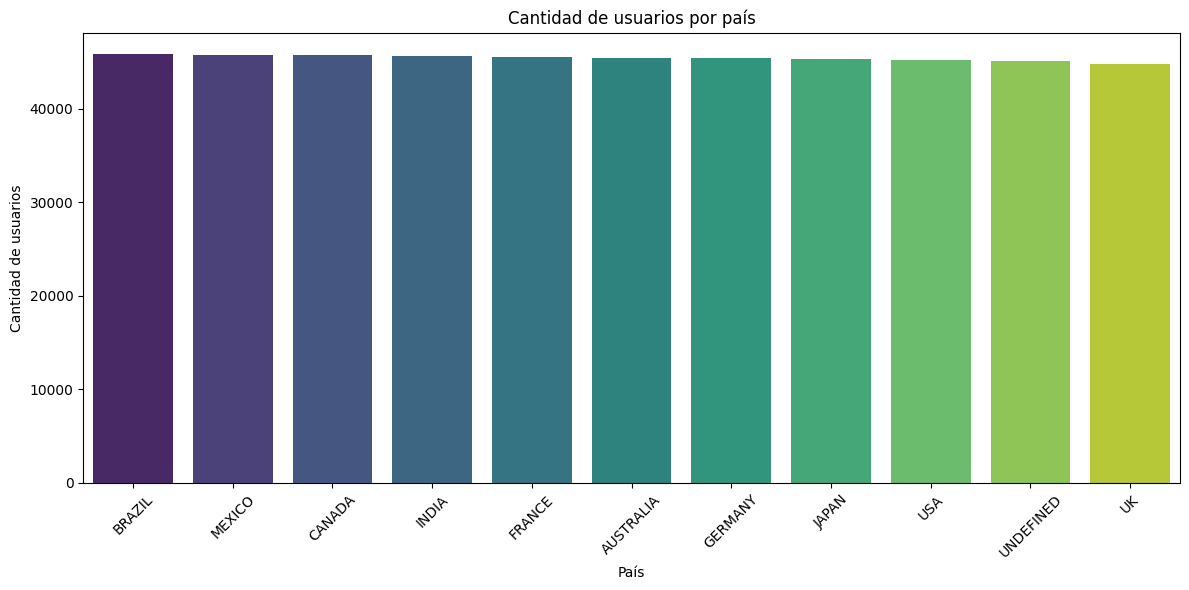
\includegraphics[width=0.8\textwidth]{imagenes/datos_uniformes/usuarios_por_pais.png}
    \caption{Cantidad de usuarios por país}
    \label{fig:usuarios_por_pais}
\end{figure}

En las siguientes dos figuras, podemos ver ilustrados los nuevos usuarios que se registran cada mes, diferenciados según el segmento al que pertenecen.
En estos gráficos se puede observar que, si bien no hay una cantidad exactamente igual de usuarios nuevos cada mes, la diferencia es muy pequeña. La mayor diferencia de nuevos usuarios está en el primer mes y el último mes registrado (ver figura \ref{fig:usuarios_nuevos_por_segmento_y_mes_de_registro}), sin embargo la proporción de nuevos usuarios respecto al total de usuarios sigue siendo muy similar en todos los meses (ver figura \ref{fig:proporcion_de_nuevos_usuarios}).

Otra cosa que se puede observar en estos gráficos es que la mayoría de los usuarios pertenecen al segmento \texttt{Regular}, mientras que los segmentos \texttt{Premium} y \texttt{Budget} son tienen menor volumen. Aún así, es destacable la proporción casi idéntica en estos últimos dos segmentos.

\begin{figure}[H]
    \centering
    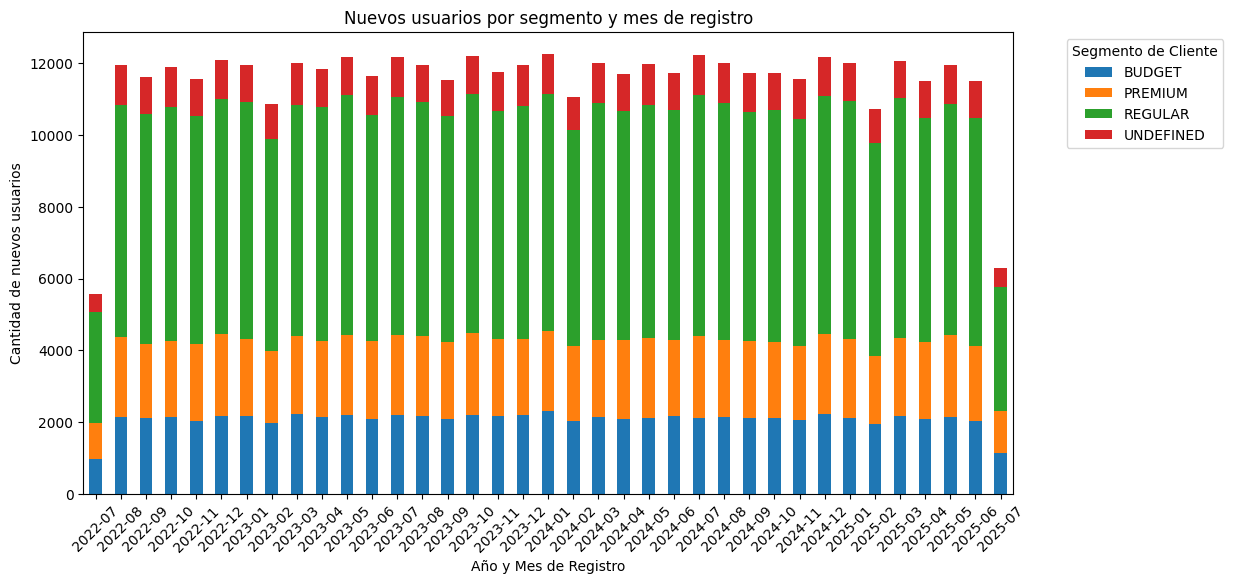
\includegraphics[width=0.8\textwidth]{imagenes/datos_uniformes/usuarios_nuevos_por_segmento_y_mes_de_registro.png}
    \caption{Cantidad de usuarios nuevos por segmento y mes de registro}
    \label{fig:usuarios_nuevos_por_segmento_y_mes_de_registro}
\end{figure}
\begin{figure}[H]
    \centering
    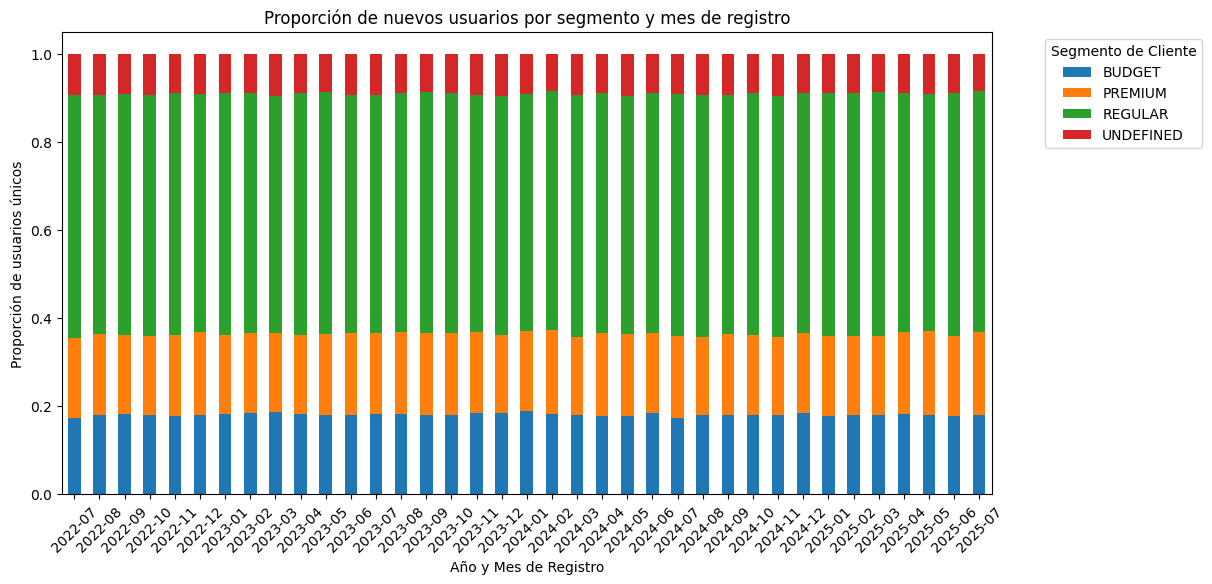
\includegraphics[width=0.8\textwidth]{imagenes/datos_uniformes/proporcion_de_nuevos_usuarios.png}
    \caption{Proporción de nuevos usuarios por segmento y mes de registro}
    \label{fig:proporcion_de_nuevos_usuarios}
\end{figure}

A continuación se muestran dos gráficos que ilustran la cantidad de usuarios por estado. En la figura \ref{fig:usuarios_por_estado} se puede observar que la mayoría de los estados tienen una cantidad similar de usuarios. En esta primera figura se visualiza una escala de 0 a 7000, y vemos que todos los estados tienen colores muy similares.

\begin{figure}[H]
    \centering
    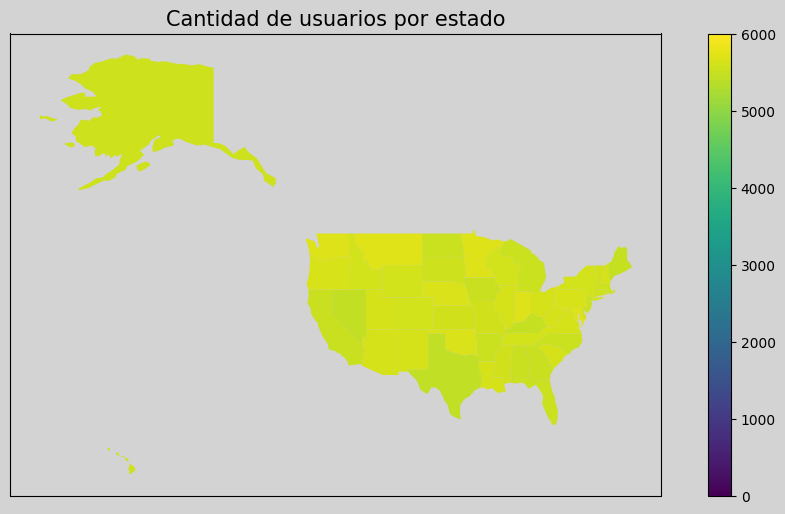
\includegraphics[width=0.8\textwidth]{imagenes/datos_uniformes/usuarios_por_estado.png}
    \caption{Cantidad de usuarios por estado}
    \label{fig:usuarios_por_estado}
\end{figure}

En la figura \ref{fig:usuarios_por_estado_closer} se puede ver el mismo mapa con una escala más cerrada, aproximadamente de 6300 a 6700. En este gráfico sí se pueden notar colores más variados. Aún así hay que notar que la diferencia entre el estado con más usuarios y el estado con menos usuarios es de a lo sumo 400 usuarios, lo cual es una diferencia bastante baja tomando en consideración el total de usuarios por estado. Esto refuerza la idea de que los datos son simulados y no representan una distribución realista de usuarios por estado. Notar como, por ejemplo, el estado de Alaska  tiene muchos más usuarios que Texas, lo cual es muy improbable en un escenario real.

\begin{figure}[H]
    \centering
    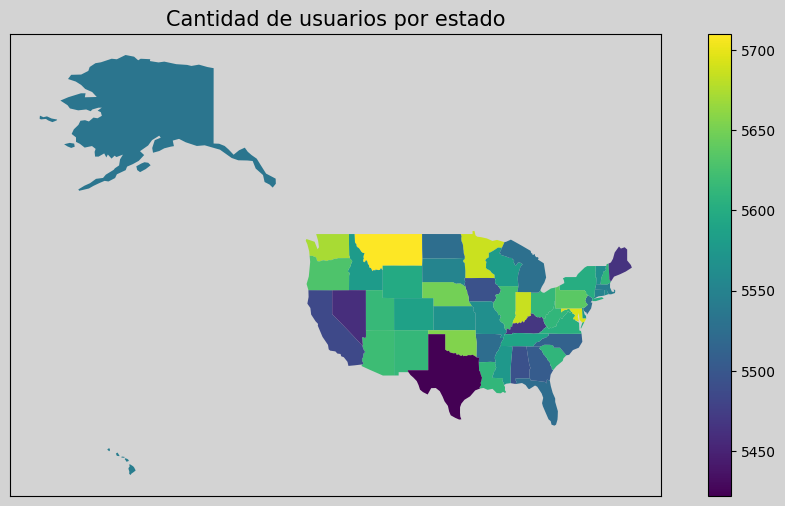
\includegraphics[width=0.8\textwidth]{imagenes/datos_uniformes/usuarios_por_estado_closer.png}
    \caption{Cantidad de usuarios por estado (detalle)}
    \label{fig:usuarios_por_estado_closer}
\end{figure}

\subsection{Órdenes}

En la figura \ref{fig:ordenes_por_estado} se pueden visualizar la cantidad de órdenes totales por estado. Nuevamente, se puede observar que la mayoría de los estados tienen una cantidad similar de órdenes, a excepción de los estados militares de Estados Unidos (AA, AE, AP) que tienen una cantidad considerablemente mayor de órdenes, casi exactamente el doble.

\begin{figure}[H]
    \centering
    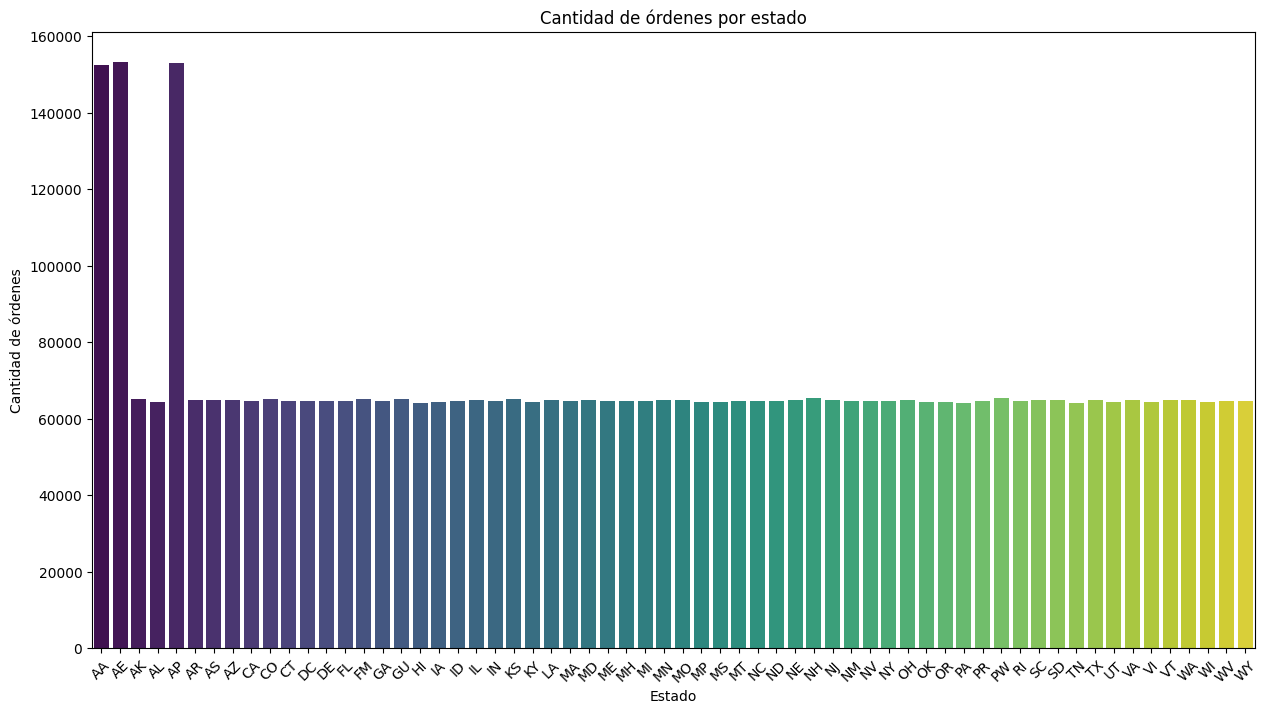
\includegraphics[width=0.8\textwidth]{imagenes/datos_uniformes/ordenes_por_estado.png}
    \caption{Cantidad de órdenes por estado}
    \label{fig:ordenes_por_estado}
\end{figure}

\begin{figure}[H]
    \centering
    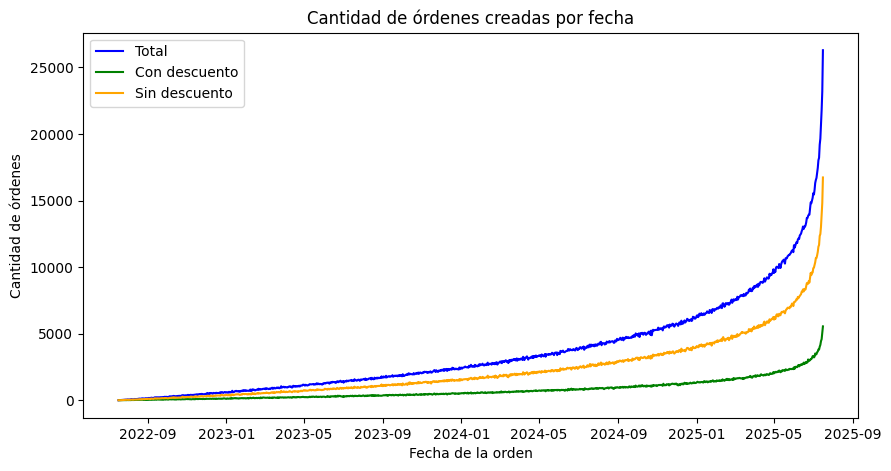
\includegraphics[width=0.8\textwidth]{imagenes/datos_uniformes/cantidad_de_ordenes_por_fecha.png}
    \caption{Cantidad de órdenes por fecha (agrupados con descuento, sin descuento y totales)}
    \label{fig:cantidad_de_ordenes_por_fecha}
\end{figure}

En la figura \ref{fig:cantidad_de_ordenes_por_fecha} se puede observar la cantidad de órdenes por fecha (i.e. la cantidad de filas en la tabla \texttt{orders} por fecha), diferenciados para órdenes con descuento, sin descuento y el total. Se puede observar que las tres curvas siguen una tendencia muy marcada, parecida a una curva exponencial, con desviaciones muy pequeñas. \\
Esto nos da una idea de cómo se pueden haber simulado los datos, podemos inferir que se utilizó algún tipo de función matemática para generar estas cifras y que se utilizó un porcentaje fijo de órdenes con descuento respecto al total de órdenes.

En la figura \ref{fig:ordenes_por_estado_en_el_tiempo} se puede observar la proporción de órdenes por estado en el tiempo. Cada color representa uno de los estados. Se puede observar nuevamente la tendencia muy marcada en todos los estados, con desviaciones muy pequeñas. Se puede apreciar muy bien cómo la cantidad de órdenes por mes es casi idéntica para todos los estados. La única excepción son las cantidades en los estados militares como se vió en la figura \ref{fig:ordenes_por_estado}, que aún puede verse que tienen que siguen una tendencia similar a la de los demás estados.

\begin{figure}[H]
    \centering
    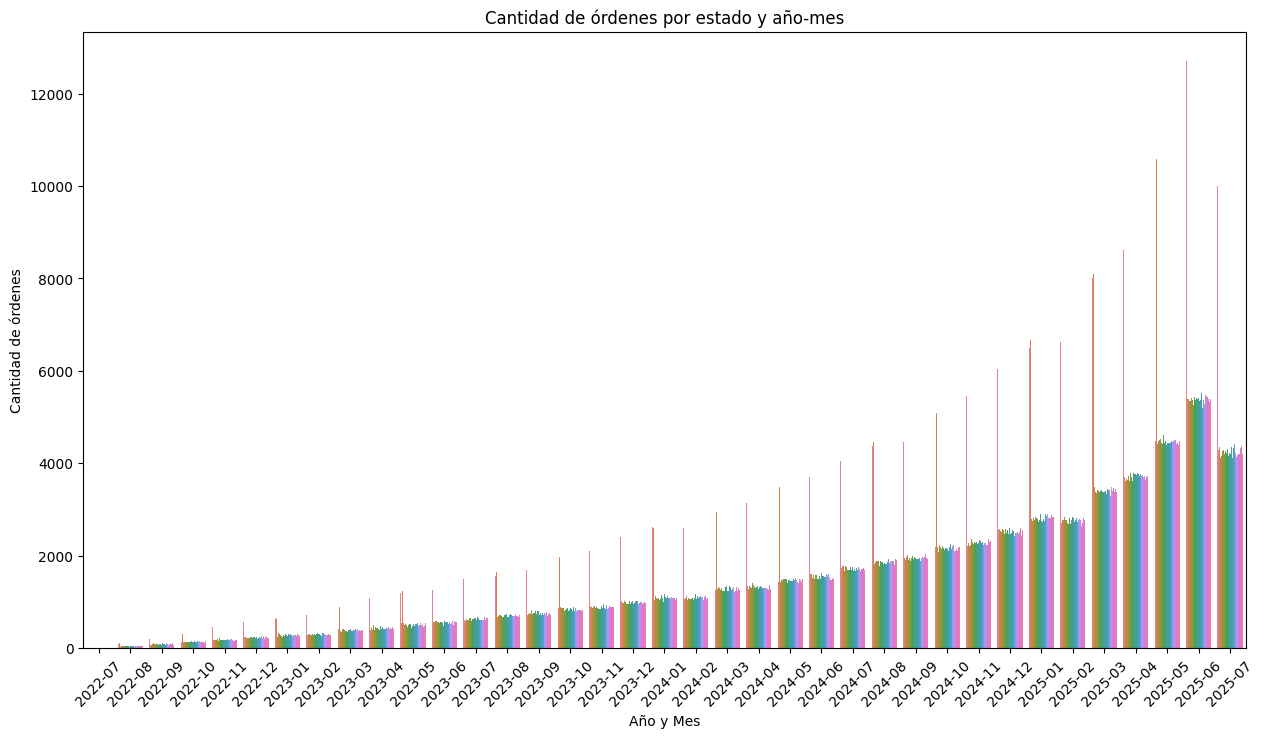
\includegraphics[width=0.8\textwidth]{imagenes/datos_uniformes/ordenes_por_estado_en_el_tiempo.png}
    \caption{Proporción de órdenes por estado en el tiempo}
    \label{fig:ordenes_por_estado_en_el_tiempo}
\end{figure}

La única anomalía en la tendencia que siguen los datos es en el último mes registrado. Esto puede deberse a que los datos fueron generados hasta una fecha específica (17/07/2025) y no se completó el mes, por lo que la cantidad de órdenes en ese mes es considerablemente menor.

\subsection{Inventario}

En la figura \ref{fig:movimientos_por_tipo_y_dia} se puede observar la cantidad de movimientos de inventario por tipo y día. Se puede observar que a lo largo del tiempo se registran cantidades de movimientos similares para cada tipo de movimiento. La única excepción es el tipo de movimiento `Undefined', que tiene una cantidad considerablemente menor de movimientos registrados.

Notar cómo se forman franjas en las cuales se distribuyen los puntos, donde cada uno representa la cantidad de movimientos que hubo en un día. Si los datos fueran reales, se podría esperar ver que las franjas sigan un ciclo anual, con más movimientos en ciertas épocas del año (por ejemplo, en diciembre por las fiestas) y menos en otras. Sin embargo, en este caso las franjas no siguen un patrón anual, sino que parecen estar distribuidas de manera uniforme a lo largo del tiempo.

\begin{figure}[H]
    \centering
    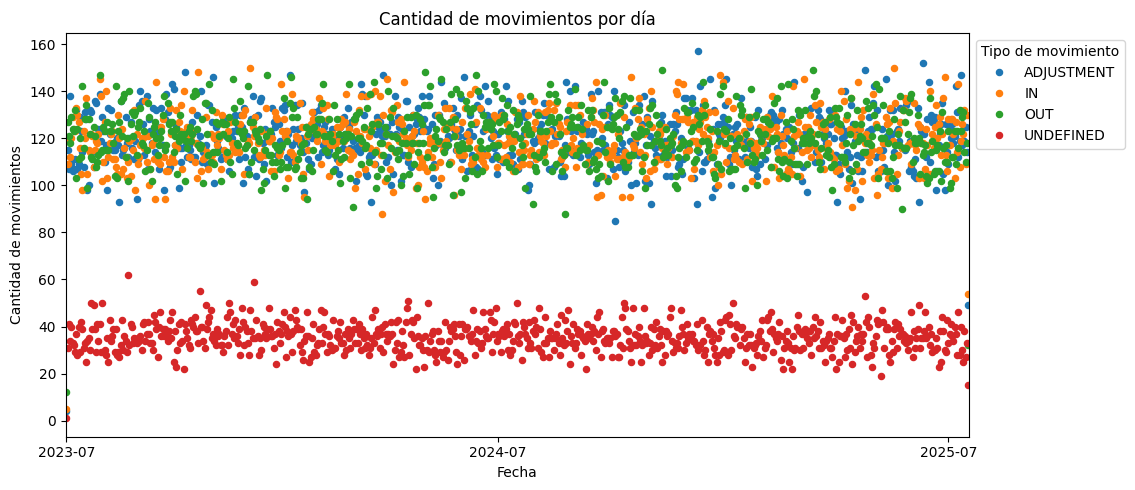
\includegraphics[width=0.8\textwidth]{imagenes/datos_uniformes/movimientos_por_tipo_y_dia.png}
    \caption{Cantidad de movimientos por tipo y día}
    \label{fig:movimientos_por_tipo_y_dia}
\end{figure}

\begin{figure}[H]
    \centering
    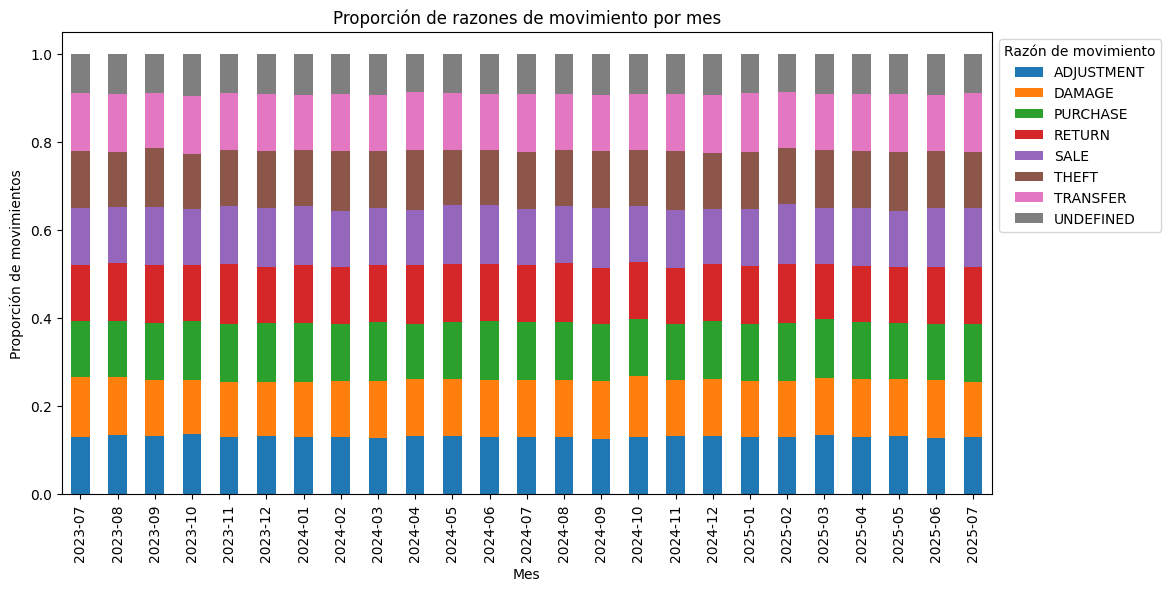
\includegraphics[width=0.8\textwidth]{imagenes/datos_uniformes/razones_de_movimientos.png}
    \caption{Proporción de razones de movimientos por mes}
    \label{fig:razones_de_movimientos}
\end{figure}

En la figura \ref{fig:razones_de_movimientos} nuevamente se puede observar una distribución uniforme en el tiempo, esta vez de las razones de movimientos de inventario. Se puede observar que hay una cantidad muy similar de todos los movimientos, y que la proporción entre ellos se mantiene casi constante a lo largo del tiempo. Por ejemplo podemos ver que la proporción entre movimientos de tipo `Sale' y `Theft' es casi exactamente 1:1 en todos los meses, lo cual sería preocupante en un escenario real.

Finalmente, se presentan dos gráficos que personalmente me gustan mucho. \\
En la figura \ref{fig:cambios_cantidad_mes} se puede observar el cambio acumulado en la cantidad de unidades del inventario (sin diferenciar entre productos). Es notable cómo la línea negra, que representa el cambio total en la cantidad, se mantiene casi constante a lo largo del tiempo, con pequeñas variaciones. Esto indica que la cantidad de unidades en el inventario no varía mucho a lo largo del tiempo. Se puede observar que en todos los meses las cantidades en los movimientos `IN' se compensan con las de los movimientos `OUT', mientras que las cantidades de los movimientos `ADJUSTMENT' y `UNDEFINED' casi no aparecen en el gráfico, lo que indica que las entradas en la tabla se cancelan entre sí en un mismo mes.

Por último, en la figura \ref{fig:distribucion_tipos_de_mov} se puede observar la distribución de los tipos de movimiento en el tiempo. Podemos observar que, aún con una elevada cantidad de \texttt{bins} en el histograma, la distribución de los tipos de movimiento es prácticamente constante para los tipos de movimiento `IN', `OUT' y `ADJUSTMENT'. Además, podemos ver límites muy marcados y redondos en los valores que toma cada tipo de movimiento. \\
También se puede observar que el tipo de movimiento `UNDEFINED' no sigue una distribución uniforme, pero sigue la misma distribución que el total de movimientos. De esta manera podemos inferir que para el dataset se crearon los datos `IN', `OUT' y `ADJUSTMENT' de manera uniforme, y luego los datos `UNDEFINED' se crearon como un porcentaje fijo del total de movimientos.

\begin{figure}[H]
    \centering
    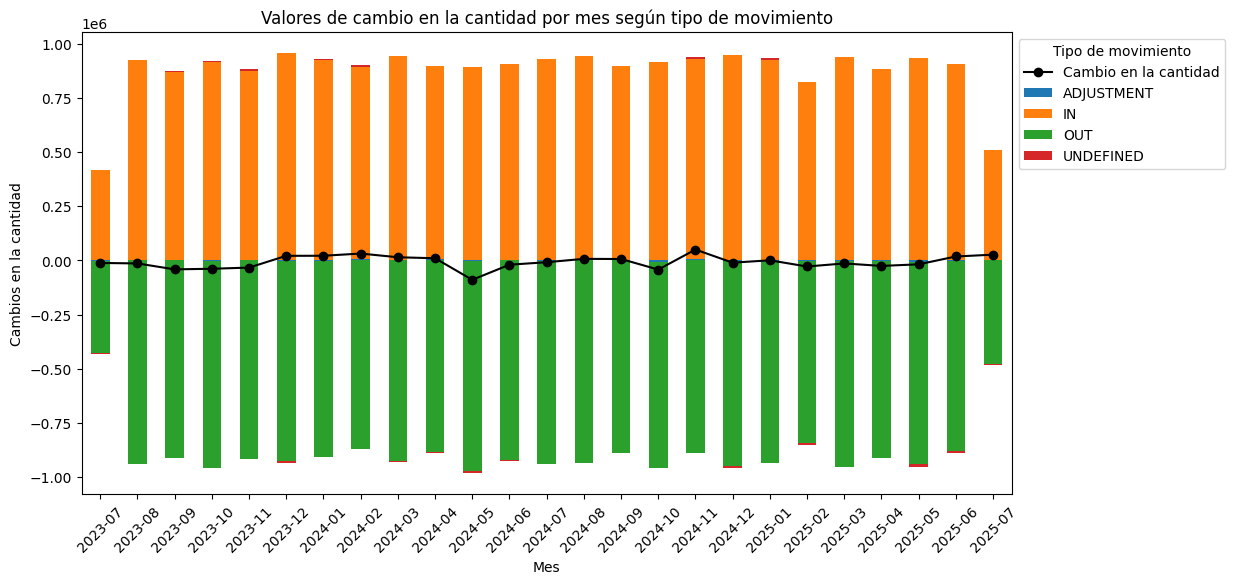
\includegraphics[width=0.8\textwidth]{imagenes/datos_uniformes/cambios_cantidad_mes.png}
    \caption{Valores de cambio en la cantidad por mes según tipo de movimiento}
    \label{fig:cambios_cantidad_mes}
\end{figure}

\begin{figure}[H]
    \centering
    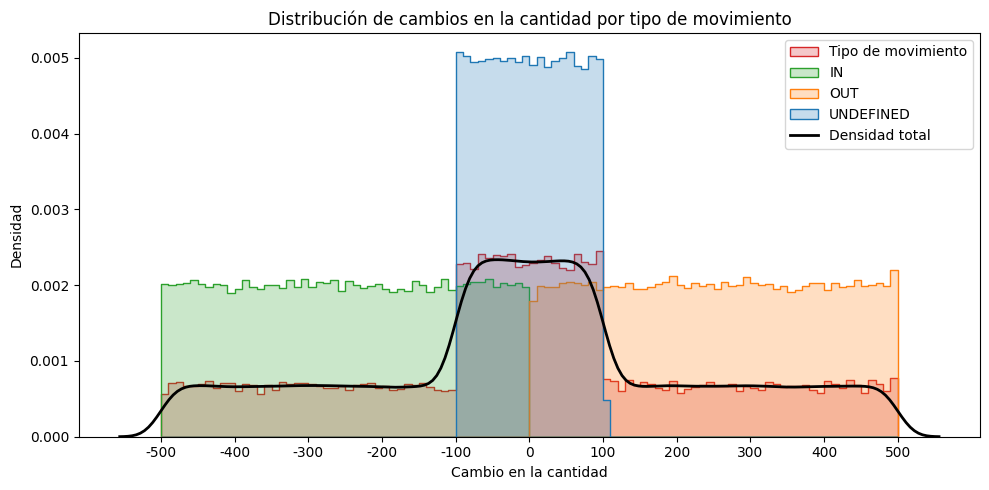
\includegraphics[width=0.8\textwidth]{imagenes/datos_uniformes/distribucion_tipos_de_mov.png}
    \caption{Distribución de valores de cambio en la cantidad según tipo de movimiento}
    \label{fig:distribucion_tipos_de_mov}
\end{figure}

    \newpage
    \section{Consultas y Visualizaciones}
    \subsection{Consultas Propuestas por el Enunciado}

\subsubsection{¿Cuál es el estado que más descuentos tiene en total? ¿y en promedio?}

Para esta consulta se tomaron algunas consideraciones:
\begin{itemize}
    \item Se consideraron los 50 Estados de los Estados Unidos. No se consideraron territorios ni estados militares.
    \item El estado a considerar es el encontrado en la columna \texttt{billing\_address} de la tabla \texttt{orders}.
    \item Se consideraron los "estados con más descuentos" a aquellos que poseen la mayor cantidad de órdenes con descuentos aplicados. Se considera que una orden tiene un descuento si el monto del descuento no es nulo y es mayor a 0.
    \item La segunda parte de la consulta (``¿y en promedio?'') se interpreta como el estado con mayor promedio en el valor de \texttt{discount\_amount}.
\end{itemize}

Para poder realizar esta consulta, fue necesario extraer el estado y el código postal de la columna \texttt{billing\_address} de la tabla \texttt{orders}. 

Las direcciones parecían seguir un patrón que me facilitó extraer el estado y el código postal mediante una expresión regular.
Para esto, primero se normalizaron los datos de la columna y luego se utilizó la siguiente expresión regular:

\begin{lstlisting}[language=Python]
orders["billing_address"] = orders["billing_address"].str.upper()
orders.fillna({"billing_address":"UNDEFINED"}, inplace=True)
pattern = r'([A-Z]{2})\s(\d{5})'
orders[["state", "zip_code"]] = orders["billing_address"].str.extract(pattern)
\end{lstlisting}

La expresión regular extrae dos grupos: el primero corresponde al estado (dos letras mayúsculas) y el segundo al código postal (cinco dígitos).
Para verificar que esta extracción fuera exitosa se realizaron las siguientes comprobaciones, para las cuales se obtuvieron resultados positivos (ver Anexo \ref{anexo:output_validacion_consulta1}).

\begin{lstlisting}[language=Python, xleftmargin=25pt, xrightmargin=25pt, ]
null_state_and_addr = orders["state"].isna() & orders["billing_address"].str.contains("UNDEFINED")

print("Todas las filas que tienen estado nulo, tienen direccion de facturacion indefinida?", 
        "Si" if null_state_and_addr.sum() == orders["state"].isna().sum() else "No")
\end{lstlisting}

Finalmente, para responder la consulta, se creó un filtro que deja fuera los estados militares y territorios llamado \texttt{not\_states\_filter} (ver Anexo \ref{anexo:output_filtro_estados}). Se filtraron las órdenes conservando solo aquellas que tenían un monto de descuento mayor a 0 y que cumplían con el filtro de estados, y se agruparon por estado, contando la cantidad de órdenes con descuento por estado.

\begin{lstlisting}[language=Python, xleftmargin=35pt, xrightmargin=35pt, ]
orders_with_discount = orders.loc[orders["discount_amount"] > 0]
                                .loc[not_states_filter]

quantity_of_orders_with_discounts_by_state = orders_with_discount.groupby("state")["order_id"]
                                                                        .count().reset_index()
\end{lstlisting}

Luego, para visualizar mejor los resultados, se renombraron las columnas y se agregó una columna con el nombre del estado utilizando \texttt{map} (ver Anexo \ref{anexo:output_formateo_resultados}). Se visualizaron los 5 estados con más órdenes utilizando la función \texttt{nlargest} de pandas.

\begin{lstlisting}[language=Python, xleftmargin=35pt, xrightmargin=35pt]
print("\nTop 5 estados con mas ordenes con descuentos:")
quantity_of_orders_with_discounts_by_state.nlargest(5, "Cantidad de Ordenes con Descuento")
\end{lstlisting}
\begin{table}[H]
\centering

\begin{tabular}{|c|c|c|}
\hline
\textbf{Código de Estado} & \textbf{Cantidad de Órdenes con Descuento} & \textbf{Nombre del Estado} \\
\hline
LA & 13,950 & Louisiana \\
MO & 13,940 & Missouri \\
IL & 13,930 & Illinois \\
KY & 13,903 & Kentucky \\
IA & 13,873 & Iowa \\
\hline
\end{tabular}
\caption{Top 5 estados con más órdenes con descuentos}
\end{table}

Entonces la respuesta a ``¿Cuál es el estado que más descuentos tiene en total?'' es Louisiana.

Luego, para encontrar el estado con mayor promedio en el valor de \texttt{discount\_amount}, se calculó el promedio del monto de descuento por estado y se utilizó nuevamente la función \texttt{nlargest} para obtener los 5 estados con mayor promedio.

\begin{lstlisting}[language=Python, xleftmargin=26pt, xrightmargin=26pt]
states_avg_discount = orders_with_discount.groupby("state")["discount_amount"].mean().reset_index()
states_avg_discount.nlargest(5, "discount_amount")
\end{lstlisting}

\begin{table}[H]
\centering
\begin{tabular}{|c|c|c|}
\hline
\textbf{Código de Estado} & \textbf{Promedio de Descuento (\$)} & \textbf{Nombre del Estado} \\
\hline
NC & 50.67 & North Carolina \\
GA & 50.46 & Georgia \\
OK & 50.42 & Oklahoma \\
CO & 50.34 & Colorado \\
MS & 50.32 & Mississippi \\
\hline
\end{tabular}
\caption{Top 5 estados con mayor promedio de monto de descuento}
\end{table}

Entonces la respuesta a ``¿y en promedio?'' es North Carolina.

\subsubsection{¿Cuáles son los 5 códigos postales más comunes para las órdenes con estado `Refunded'? ¿Y cuál es el nombre más frecuente entre los clientes de esas direcciones?}

Para resolver esta consulta, se aprovechó la extracción del código postal realizada sobre la tabla \texttt{orders} en la consulta anterior. 
En primer lugar, se filtraron las órdenes con estado `Refunded` y se contaron la cantidad de órdenes por código postal utilizando la función \texttt{value\_counts}. Luego, se utilizó las función \texttt{nlargest} para obtener los 5 códigos postales más comunes entre las órdenes con estado `Refunded`.

\begin{lstlisting}[language=Python, xleftmargin=35pt, xrightmargin=35pt]
refunded_orders = orders[orders["status"].str.contains("REFUNDED")]

amount_refunded_orders_by_zipcode = refunded_orders["zip_code"].value_counts().reset_index()
top_refunded_zipcodes = amount_refunded_orders_by_zipcode.nlargest(5, "count")

print("\nTop 5 codigos postales mas comunes para ordenes con estado 'Refunded':")
print(top_refunded_zipcodes)
\end{lstlisting}
\begin{table}[H]
\centering
\begin{tabular}{|c|c|}
\hline
\textbf{Código Postal} & \textbf{Cantidad de Órdenes `Refunded`} \\
\hline
31571 & 6 \\
65247 & 5 \\
38151 & 5 \\
09045 & 5 \\
14396 & 5 \\
\hline
\end{tabular}
\caption{Top 5 códigos postales más comunes para órdenes con estado `Refunded`}
\end{table}
Como los puestos 2, 3, 4 y 5 están empatados con 5 órdenes cada uno, se agregó una consulta adicional para ver todos los códigos postales que tienen 5 órdenes `Refunded` (ver Anexo \ref{anexo:output_codigos_postales_refunded}).

Para obtener los nombres más frecuentes entre los clientes de esos códigos postales, se filtró la tabla \texttt{customers} utilizando el método \texttt{isin} para seleccionar únicamente las filas cuyo \texttt{postal\_code} se encuentra en un conjunto específico de valores. Luego se contaron las apariciones de cada nombre utilizando nuevamente la función \texttt{value\_counts}. Para mostrar los 5 nombres más frecuentes, se utilizó la función \texttt{nlargest}.

\begin{lstlisting}[language=Python, xleftmargin=20pt, xrightmargin=20pt]
most_common_names = customers
    .loc[customers["postal_code"].isin(top_refunded_zipcodes["zip_code"])]["first_name"].value_counts()
most_common_names.nlargest(5)
\end{lstlisting}
\begin{table}[H]
\centering
\begin{tabular}{|c|c|}
\hline
\textbf{Nombre} & \textbf{Cantidad de Apariciones} \\
\hline
UNDEFINED & 4 \\
RICHARD & 2 \\
MICHAEL & 2 \\
ROBERT & 1 \\
CYNTHIA & 1 \\
\hline
\end{tabular}
\caption{Top 5 nombres más frecuentes entre los clientes de los códigos postales con más órdenes `Refunded`}
\end{table}

Como puede verse, el nombre más frecuente entre los clientes de esas direcciones es `UNDEFINED`, que aparece 4 veces. Esto significa que hay 4 órdenes registradas por clientes sin nombre registrado. Nuevamente, se realizó una consulta adicional para ver otros nombres que aparecen una sola vez (ver Anexo \ref{anexo:nombres_mas_comunes}).

\subsubsection{Para cada tipo de pago y segmento de cliente, devolver la suma y el promedio expresado como porcentaje, de clientes activos y de consentimiento de marketing.}

Para resolver esta consulta era necesario tener columnas tanto en la tabla \texttt{customers} como en la tabla \texttt{orders}. Por lo tanto, se realizó un \texttt{merge} entre ambas tablas utilizando la columna \texttt{customer\_id} como clave.

\begin{lstlisting}[language=Python, xleftmargin=78pt, xrightmargin=78pt]
orders_customers = orders.merge(customers, on="customer_id").reset_index()
\end{lstlisting}

Luego, para evitar contar dos veces a un mismo cliente que hizo varias órdenes con el mismo método de pago, se eliminaron las filas duplicadas basándose en las columnas \texttt{customer\_id} y \texttt{payment\_method}. 

\begin{lstlisting}[language=Python, xleftmargin=23pt, xrightmargin=23pt]
orders_customers_unique = orders_customers.drop_duplicates(subset=["payment_method", "customer_id"])
\end{lstlisting}

Finalmente, se agrupó por \texttt{payment\_method} y \texttt{customer\_segment}, y se calcularon las funciones de agregación necesarias para obtener la cantidad total de clientes, la cantidad de clientes activos y la cantidad de clientes con consentimiento de marketing. Luego, se calcularon los promedios expresados como porcentaje.

\begin{lstlisting}[language=Python, xleftmargin=100pt, xrightmargin=100pt]
orders_customers_grouped = orders_customers_unique
    .groupby(["payment_method", "customer_segment"]).agg({
        "customer_id": "count",
        "is_active": ["sum", "mean"],
        "marketing_consent": ["sum", "mean"]
    })
orders_customers_grouped[('is_active', 'mean')] *= 100
orders_customers_grouped[('marketing_consent', 'mean')] *= 100
\end{lstlisting}

Me pareció interesante graficar los resultados utilizando un \texttt{heatmap} de la librería \texttt{seaborn}, para lo cual fue necesario reestructurar el DataFrame utilizando la función \texttt{unstack} (ver Anexo \ref{anexo:consulta3_heatmap}). En el notebook también pueden encontrarse los resultados expuestos como tabla.

\subsubsection{Para los productos que contienen en su descripción la palabra `stuff', calcular el peso total de su inventario agrupado por marca}

Para esta consulta, se asumió que la columna \texttt{weight\_kg} representa el peso unitario del producto en el inventario.

Primero se filtraron los productos que contienen la palabra `stuff' en su descripción, sin importar mayúsculas o minúsculas. Para esto se utilizó el método \texttt{str.contains} de pandas, con el parámetro \texttt{case=False} para ignorar mayúsculas y minúsculas. También se seleccionaron únicamente las columnas relevantes para la consulta: \texttt{brand}, \texttt{weight\_kg} y \texttt{stock\_quantity}.

\begin{lstlisting}[language=Python, xleftmargin=0pt, xrightmargin=0pt]
stuff_products = products
    .loc[products["description"].str.contains("STUFF", case=False)][["brand", "weight_kg", "stock_quantity"]]
\end{lstlisting}

Luego, se calculó el peso total de cada producto multiplicando el peso unitario por la cantidad en stock, y se creó una nueva columna llamada \texttt{total\_weight\_kg}. También se eliminaron las columnas que ya no eran necesarias.

\begin{lstlisting}[language=Python, xleftmargin=25pt, xrightmargin=25pt]
stuff_products["total_weight_kg"] = stuff_products["weight_kg"] * stuff_products["stock_quantity"]
stuff_products.drop(columns=["weight_kg", "stock_quantity"], inplace=True)
\end{lstlisting}

Finalmente, se agrupó por marca y se sumó el peso total de los productos de cada marca. Se utilizó la función \texttt{nlargest} para obtener las 5 marcas con mayor peso total en inventario.

\begin{lstlisting}[language=Python, xleftmargin=75pt, xrightmargin=75pt]
    stuff_products.groupby("brand")["total_weight_kg"].sum().nlargest(5)
\end{lstlisting}

\begin{table}[H]
\centering
\begin{tabular}{|c|c|}
\hline
\textbf{Marca} & \textbf{Peso Total (kg)} \\
\hline
UNDEFINED & 11,157,882.66 \\
3M & 2,250,899.67 \\
ADIDAS & 1,923,907.88 \\
NIKE & 1,783,569.90 \\
HASBRO & 1,714,411.24 \\
\hline
\end{tabular}
\caption{Top 5 marcas con mayor peso total de productos con 'stuff' en la descripción}
\end{table}

    \subsection{Consultas Propias}
    A continuación se presentan consultas adicionales para cumplir con los requerimientos del trabajo práctico, junto con las consideraciones tomadas para su resolución y los resultados obtenidos. El código fuente y los resultados completos pueden encontrarse en el notebook \href{https://github.com/patricioibar/datos-tp1/blob/main/consultas_propias.ipynb}{\texttt{consultas\_propias.ipynb}}.

Las siguientes consultas fueron realizadas intentando cubrir las visualizaciones que se piden en la propuesta del trabajo práctico. Estas requieren la comparación de los siguientes tipos de variables:
\begin{enumerate}
    \item Una continua con una línea de tiempo.
    \item Una discreta con una continua.
    \item Una discreta con una discreta.
    \item Una continua con otra continua.
\vspace{-1em}
\end{enumerate}
Además, se agregaron las siguientes visualizaciones adicionales:
\vspace{-1em}
\begin{enumerate}
    \setcounter{enumi}{4}
    \item Un heatmap.
    \item Línea de regresión.
    \item Boxplot.
    \item Treemap.
\end{enumerate}

Estas consultas están ideadas para intentar extraer información útil del dataset, aunque resulte imposible por su característica uniformidad.

\subsubsection{Evolución del ingreso neto de dólares a lo largo del tiempo}

Para calcular el ingreso neto de dólares, utilicé la tabla \texttt{orders} que contiene el tipo de cambio utilizado en cada orden.\\
Consideré el ingreso neto como la diferencia entre el total pagado por orden y el total de descuentos e impuestos aplicados. La fórmula que surge es la siguiente:
\[\texttt{Ingreso Neto} = \texttt{Total Pagado} - \texttt{Descuentos} - \texttt{Impuestos}\]

Para conseguir una evolución a lo largo del tiempo y poder graficarlo como una variable continua, agrupé los datos por fecha de creación de la orden, sumando las columnas de ingreso neto.

\begin{lstlisting}[language=Python, xleftmargin=25pt, xrightmargin=25pt]
data = orders.loc[orders.currency == "USD"][["date","total_amount","discount_amount","tax_amount"]]
data["net_income"] = data["total_amount"] - data["discount_amount"] - data["tax_amount"]
data = data.groupby("date")["net_income"].sum().reset_index()
\end{lstlisting}

\begin{figure}[H]
    \centering
    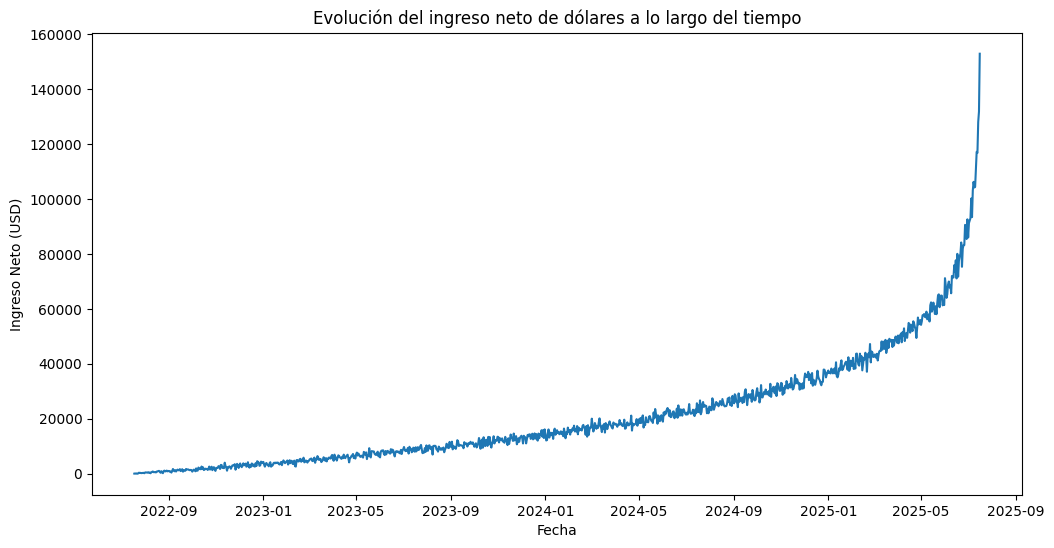
\includegraphics[width=0.8\textwidth]{imagenes/consultas_propias/evolucion_ingreso_neto.png}
    \caption{Evolución del ingreso neto de dólares a lo largo del tiempo.}
    \label{fig:ingreso_neto}
\end{figure}

Puede observarse en la figura \ref{fig:ingreso_neto} que el ingreso neto de dólares ha tenido una tendencia creciente muy marcada a lo largo del tiempo, similar a la encontrada en la figura \ref{fig:cantidad_de_ordenes_por_fecha}. Esto nos da la idea que el ingreso neto aumenta a medida que aumenta la cantidad de órdenes.

\subsubsection{Cantidad de dólares gastados por método de pago por clientes militares activos}

Se considera que un cliente es `militar' si su dirección tiene el estado `AA', `AE' o `AP'. Además, se considera que un cliente es `activo' si la columna \texttt{is\_active} de la tabla \texttt{customers} es verdadera.

Primero filtré los clientes que tienen direcciones militares y que tienen la columna \texttt{is\_active} en verdadero, y conservé únicamente los IDs de los clientes. Luego, filtré la tabla \texttt{orders} para quedarme con las órdenes realizadas por estos clientes y que estén en dólares, utilizando un llamado a \texttt{loc} y otro a \texttt{merge}. Finalmente, agrupé por método de pago y sumé el total gastado.

\begin{lstlisting}[language=Python, xleftmargin=25pt, xrightmargin=25pt]
military_states = ['AA', 'AE', 'AP']
active_military_customers = customers
        .loc[(customers['is_active']) & (customers['state'].isin(military_states))]['customer_id']
        .reset_index()

active_military_orders = orders
        .loc[orders.currency == "USD"]
        .merge(active_military_customers, on='customer_id', how='inner')
        
payment_method_sum = active_military_orders.groupby('payment_method')['total_amount'].sum()
\end{lstlisting}

\begin{figure}[H]
    \centering
    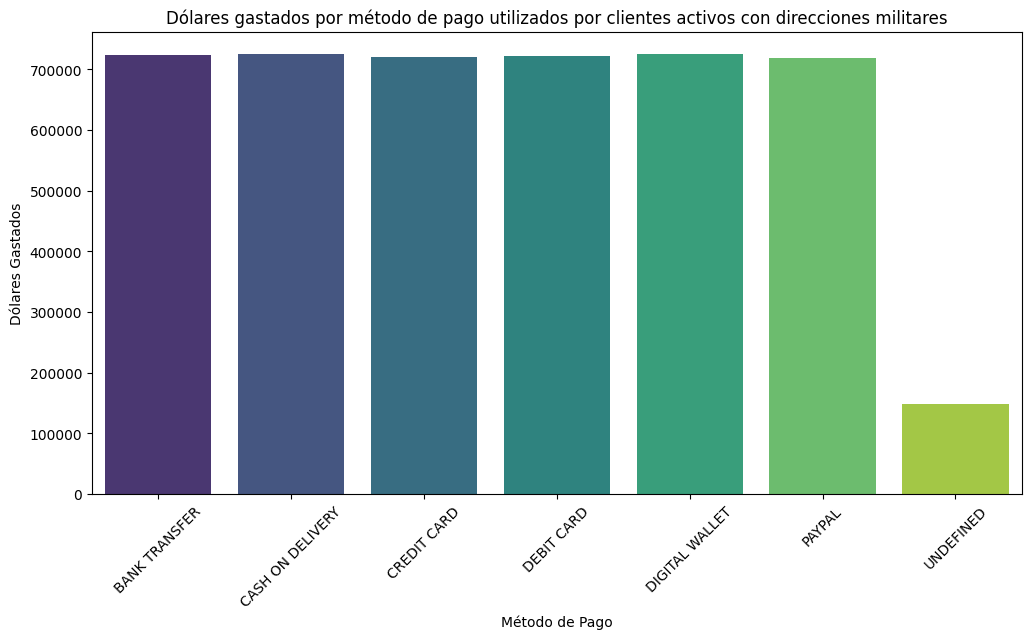
\includegraphics[width=0.8\textwidth]{imagenes/consultas_propias/dolares_militares.png}
    \caption{Cantidad de dólares gastados por método de pago por clientes activos con direcciones militares.}
    \label{fig:dolares_militares}
\end{figure}

Podemos observar una cantidad similar de dólares gastados en cada método de pago, solamente notando una diferencia notable en el método de pago `undefined', que tiene un gasto considerablemente menor.

\subsubsection{Distribución de calificaciones según segmento de cliente.}

Para esta consulta combiné las tablas \texttt{customers} y \texttt{reviews} utilizando un llamado a \texttt{merge}, ya que necesitaba la columna \texttt{customer\_segment} de la tabla \texttt{customers} y la columna \texttt{rating} de la tabla \texttt{reviews}. \\
Luego, para calcular la distribución de calificaciones debería contar las apariciones de cada calificación (de 1 a 5) por cada segmento de cliente y luego dividir por el total de reviews en ese segmento. Encontré que esto puede hacerse utilizando únicamente el método \texttt{value\_counts} estableciendo como verdadero el parámetro \texttt{normalize}.
\begin{lstlisting}[language=Python, xleftmargin=20pt, xrightmargin=20pt]
reviews = reviews.merge(customers[['customer_id', 'customer_segment']], on='customer_id', how='left')
reviews.fillna({'customer_segment': 'UNDEFINED'}, inplace=True)
data = reviews.groupby('customer_segment')['rating'].value_counts(normalize=True).unstack()
\end{lstlisting}
Decidí completar los valores faltantes en la columna \texttt{customer\_segment} con el valor `UNDEFINED', ya que no se puede inferir de ninguna manera el valor para esa columna, pero aún quería conservar todas las reviews en el análisis. 

\begin{figure}[H]
    \centering
    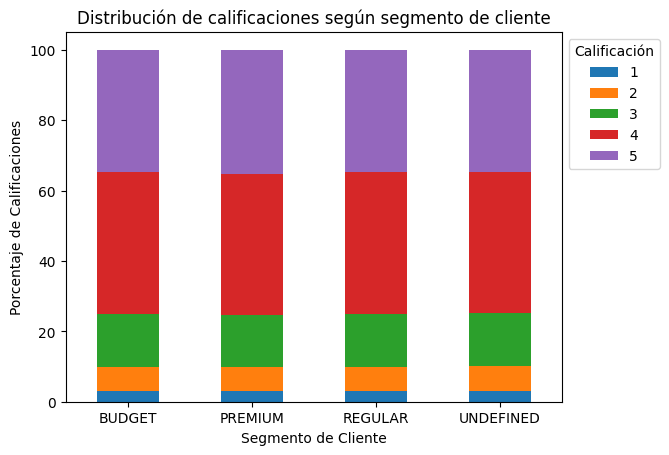
\includegraphics[width=0.8\textwidth]{imagenes/consultas_propias/calificaciones_segmentos.png}
    \caption{Distribución de calificaciones según segmento de cliente.}
    \label{fig:distribucion_calificaciones}
\end{figure}

Pueden observarse nuevamente distribuciones muy uniformes, sin una diferencia notable entre los segmentos de clientes. Puede identificarse que la mayoría de calificaciones son de 4 y 5 estrellas, y que las calificaciones de 1 estrella son las menos frecuentes.

\subsubsection{Relación entre stock disponible y ventas de unidades de zapatos}

Realicé esta consulta con la idea de poder ver si existe alguna relación entre la cantidad de stock disponible y la cantidad de unidades vendidas de zapatos. Quería ver si a mayor stock disponible, mayor cantidad de ventas, o si por el contrario no existe una relación entre estas variables.

Para esto, consideré que el stock encontrado en la tabla de \texttt{products} es el stock actual del producto. Se compara contra las ventas históricas de unidades de ese producto, que se encuentran en la tabla \texttt{order\_items}. No fue posible filtrar según tiempos de ventas, ya que esa información no se encuentra en la tabla \texttt{order\_items}, y no es posible cruzar esta tabla con la tabla \texttt{orders} ya que no identificadores de órdenes en común.

Para realizar esta consulta primero identifiqué los IDs de las categoráis de zapatos, y los utilicé para buscar los IDs de los productos que pertenecen a estas categorías. Luego, utilicé estos IDs para filtrar la tabla \texttt{order\_items} y quedarme con las ventas de unidades de zapatos. Agrupé por ID de producto y sumé la cantidad de unidades vendidas. Finalmente, realicé un \texttt{merge} con la tabla \texttt{products} para obtener el stock disponible de cada producto, y con la previemante generada \texttt{shoes\_categories} para obtener los nombres de las categorías.

\begin{figure}
\begin{lstlisting}[language=Python, xleftmargin=10pt, xrightmargin=10pt]
shoes_categories = categories[categories['parent_category'] == 'SHOES'][['category_id', 'category_name']]
shoes_products = products[products['category_id'].isin(shoes_categories['category_id'])]

shoes_order_items = items[items['product_id'].isin(shoes_products['product_id'])]
.groupby('product_id')['quantity'].sum().reset_index()

data = shoes_order_items.merge(
products[['product_id', 'stock_quantity', 'category_id']], on='product_id', how='left'
)
data = data.merge(
shoes_categories[['category_id', 'category_name']], on='category_id', how='left'
)
\end{lstlisting}
\end{figure}

Me pareció curioso que al graficar esto en un scatter plot, la leyenda de colores no contenía únicamente las categorías de zapatos, sino que también aparecían categorías de otros tipos de productos. Esto se debía a que la columna \texttt{category\_name} es de tipo \texttt{category} y aún luego de ser filtrada y mergeada, conservaba los valores originales. Para solucionar esto, convertí la columna a tipo \texttt{string}.

\begin{figure}[H]
    \centering
    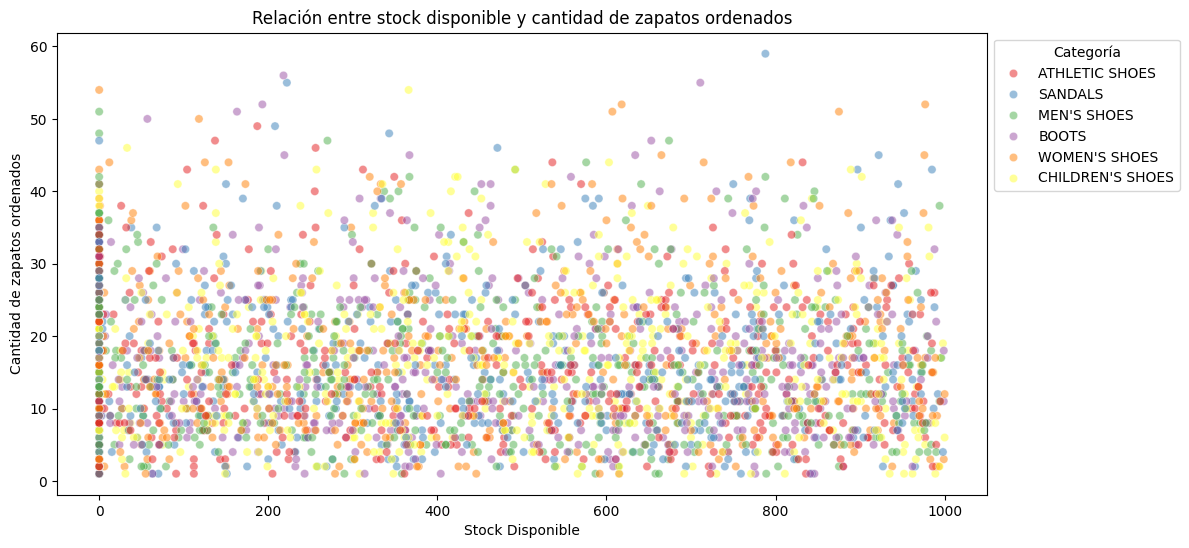
\includegraphics[width=0.8\textwidth]{imagenes/consultas_propias/stock_zapatos.png}
    \caption{Relación entre stock disponible y ventas de unidades de zapatos.}
    \label{fig:stock_vs_ventas}
\end{figure}

Lamentablemente, no se observa una relación clara entre las variables. Tampoco se puede observar una diferencia clara entre el comportamiento de las distintas categorías de zapatos.\\
Puede observarse una concentración elevada en los puntos en el valor de x=0, que indica que hay muchos productos de zapatos que no tienen stock.

\subsubsection{Rating promedio por categoría padre y segmento de cliente}

Para esta consulta combiné las tablas \texttt{reviews}, \texttt{products}, \texttt{categories} utilizando llamados a \texttt{merge}, ya que necesitaba la columna \texttt{rating} de la tabla \texttt{reviews}, la columna \texttt{category\_id} de la tabla \texttt{products}, la columna \texttt{parent\_category} de la tabla \texttt{categories}. También necesitaba la columna \texttt{customer\_segment} de la tabla \texttt{customers}, que ya se encontraba en la tabla \texttt{reviews} una consulta anterior.\\
Luego agrupé por categoría padre y segmento de cliente, y calculé el promedio de las calificaciones.
\begin{lstlisting}[language=Python, xleftmargin=20pt, xrightmargin=20pt]
reviews = reviews.merge(products[['product_id', 'category_id']], on='product_id', how='left')
reviews = reviews.merge(categories[['category_id', 'parent_category']], on='category_id', how='left')
data = reviews.groupby(['parent_category', 'customer_segment'])['rating'].mean().unstack()
\end{lstlisting}

\begin{figure}[H]
    \centering
    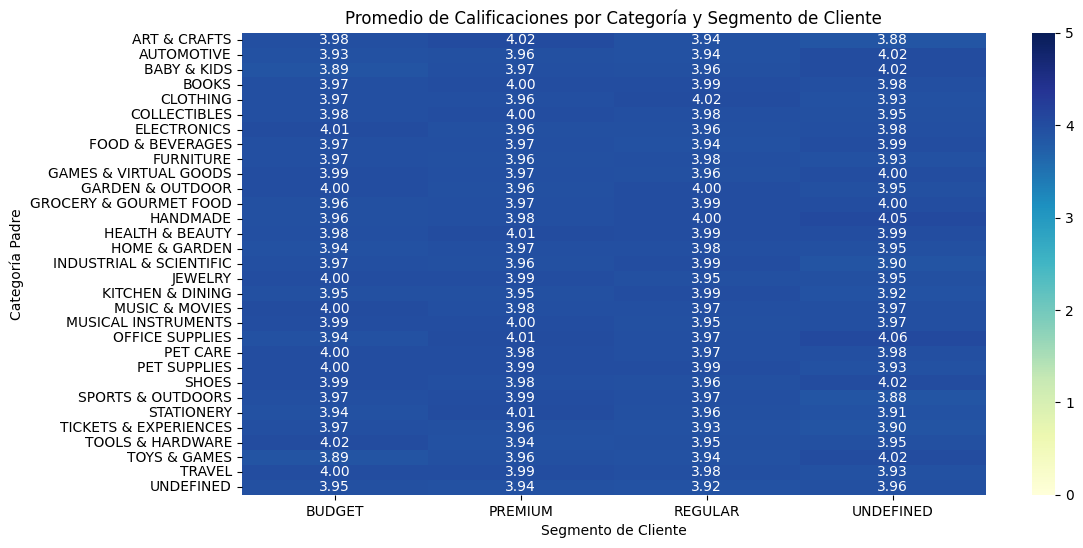
\includegraphics[width=0.8\textwidth]{imagenes/consultas_propias/rating_promedio_padre.png}
    \caption{Rating promedio por categoría padre y segmento de cliente.}
    \label{fig:rating_promedio}
\end{figure}
\vspace{-1em}
\begin{figure}[H]
    \centering
    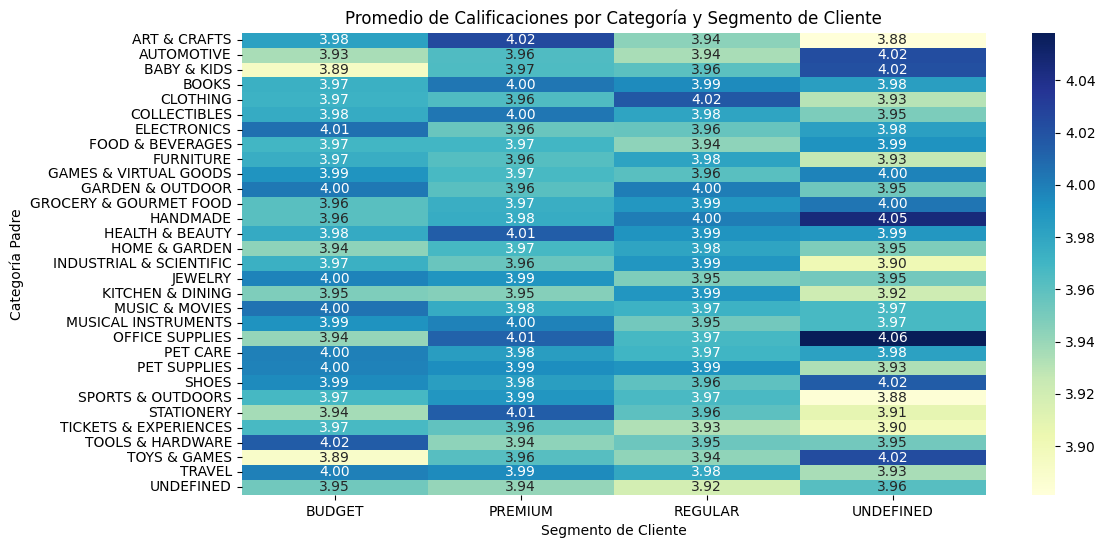
\includegraphics[width=0.8\textwidth]{imagenes/consultas_propias/rating_promedio_padre_closer.png}
    \caption{Rating promedio por categoría padre y segmento de cliente, con una escala de color más cercana.}
    \label{fig:rating_promedio_closer}
\end{figure}
Puede observarse en la figura \ref{fig:rating_promedio} que todos los ratings promedio se encuentran muy cercanos a 4, obteniendo un heatmap de color casi uniforme. \\
En la figura \ref{fig:rating_promedio_closer} se ajusta la escala de colores para poder observar mejor las diferencias entre los ratings promedio. La escala va aproximadamente desde 3.85 hasta 4.10, lo cual es bastante pequeño. Aún con esta escala ajustada, se pueden observar que la mayoría de ratings se encuentran muy cercanos entre sí.

\subsubsection{Relación entre precio de Smartphones activos y sus unidades vendidas}

Originalmente, esta consulta se había planteado como la relación entre el precio de smartphones activos y su rating promedio. Sin embargo, como se observó en consultas anteriores, los ratings promedio de los productos se encuentran todos muy cercanos entre sí, por lo que no sería posible observar una relación clara entre estas variables. Por este motivo, se decidió cambiar la variable a comparar contra el precio por la cantidad de unidades vendidas.

Para realizar esta consulta, primero identifiqué el ID de la categoría `SMARTPHONES', y lo utilicé para buscar los IDs de los productos que pertenecen a esta categoría y que además están activos. Luego, utilicé estos IDs para filtrar la tabla \texttt{order\_items} y agrupé por ID de producto para sumar la cantidad de unidades vendidas. Finalmente, realicé un \texttt{merge} con la tabla \texttt{products} para obtener el precio de cada producto.

\begin{lstlisting}[language=Python, xleftmargin=40pt, xrightmargin=40pt]
smartphone_category_id = categories[
    categories['category_name'] == 'SMARTPHONES'
    ]['category_id'].iloc[0]

active_smartphones = products[
    (products['category_id'] == smartphone_category_id) & (products['is_active'])
    ][['product_id', 'price']]

data = items[items['product_id'].isin(active_smartphones['product_id'])]
            .groupby('product_id')['quantity'].sum().reset_index()

data = data.merge(active_smartphones[['product_id', 'price']], on='product_id', how='left')
\end{lstlisting}

\begin{figure}[H]
    \centering
    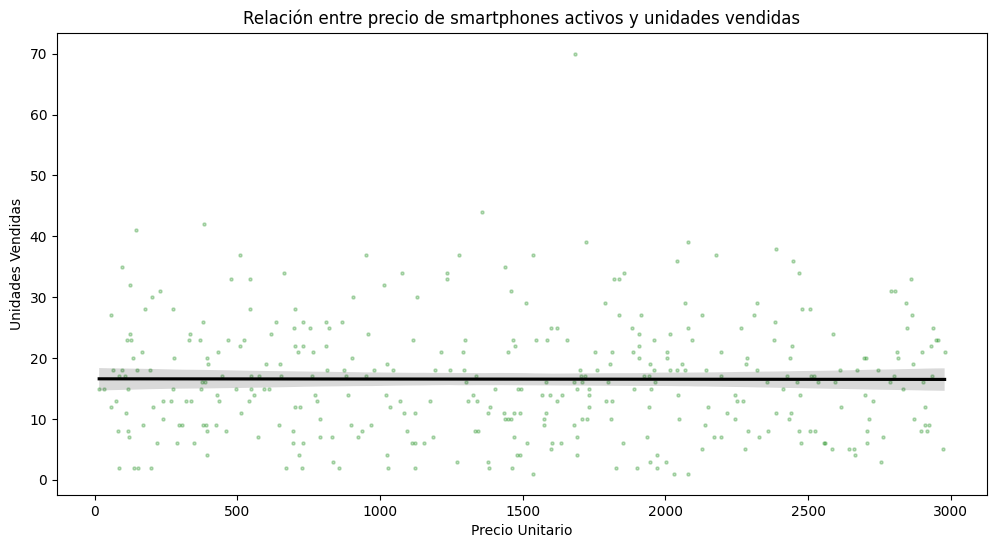
\includegraphics[width=0.8\textwidth]{imagenes/consultas_propias/smartphones.png}
    \caption{Relación entre precio de smartphones activos y unidades vendidas.}
    \label{fig:smartphone_price_vs_quantity}
\end{figure}

Una vez más, la distribución de los puntos es bastante uniforme, sin una relación clara entre las variables. No se observa que a mayor precio, mayor o menor cantidad de unidades vendidas. Más aún, puede observarse que la línea de regresión es prácticamente horizontal, indicando que no existe una relación lineal entre las variables sino que se distribuyen de manera uniforme.

\subsubsection{Distribución del descuento unitario para las 5 categorías de producto más vendidas}

Para hallar el descuento unitario de la venta de un producto, supuse que la columna \texttt{discount\_amount} de la tabla \texttt{order\_items} representa el descuento total aplicado a la venta de ese producto en esa orden. Por lo tanto, el descuento unitario puede hallarse dividiendo este valor por la cantidad de unidades vendidas de ese producto en esa orden.

Primero encontré las 5 categorías de productos más vendidas sumando la cantidad de unidades vendidas por categoría. Para esto, realicé un \texttt{merge} entre las tablas \texttt{order\_items} y \texttt{products} para poder obtener el ID de la categoría de cada producto vendido. Aproveché este  paso para quedarme únicamente con las columnas que voy a utilizar en esta consulta. Luego, agrupé por ID de categoría y sumé la cantidad de unidades vendidas, quedándome con las 5 categorías con mayor cantidad de ventas utilizando \texttt{nlargest}. \\
Luego, filtré las filas de la tabla \texttt{order\_items} para quedarme únicamente con los productos que pertenecen a estas categorías, para poder visuaizar la distribución de esos valores. Finalmente, calculé el descuento unitario y graficé su distribución utilizando violinplot.

\begin{lstlisting}[language=Python, xleftmargin=19pt, xrightmargin=19pt]
items_categories = items.merge(
    products[['product_id', 'category_id']], on='product_id', how='left'
    )[['product_id', 'category_id', 'quantity', 'discount_amount']]

top_5_categories = items_categories.groupby('category_id')['quantity'].sum().nlargest(5)

items_categories = items_categories[items_categories['category_id'].isin(top_5_categories.index)]
items_categories['unit_discount'] = items_categories['discount_amount'] / items_categories['quantity']
\end{lstlisting}

Para quedarme con los nombres de las categorías en lugar de sus IDs, armé un diccionario a partir de la tabla \texttt{categories} y utilicé el método \texttt{map} para crear una nueva columna con los nombres.

\begin{lstlisting}[language=Python, xleftmargin=35pt, xrightmargin=35pt]
categories_names = categories[['category_id', 'category_name']]
    .loc[categories['category_id'].isin(top_5_categories.index)].reset_index()

    category_name_map = {}
for _, row in categories_names.iterrows():
    category_name_map[row['category_id']] = row['category_name']

items_categories['category_id'] = items_categories['category_id'].map(category_name_map)
items_categories.rename(columns={'category_id': 'category_name'}, inplace=True)
\end{lstlisting}

También reemplacé los valores nulos de la columna \texttt{unit\_discount} por 0, ya que supuse que estos valores se producen cuando no hubo descuento aplicado en la venta del producto.

\begin{figure}[H]
    \centering
    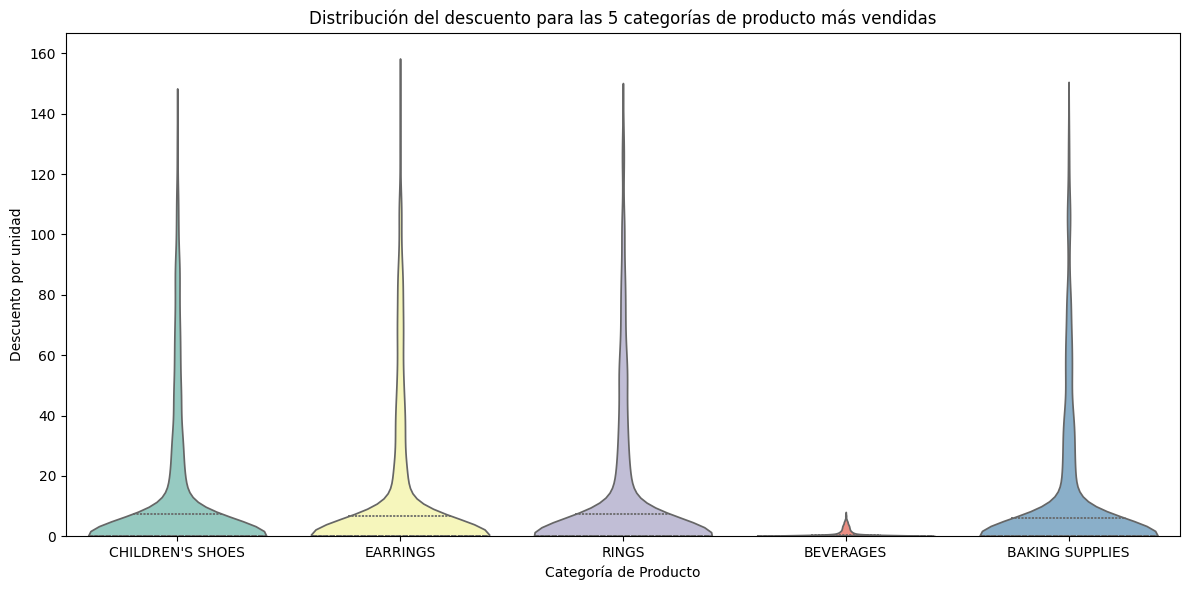
\includegraphics[width=0.8\textwidth]{imagenes/consultas_propias/descuento_categorias.png}
    \caption{Distribución del descuento unitario para las 5 categorías de producto más vendidas.}
    \label{fig:descuento_categorias}
\end{figure}

Mostré los violin plots `truncados' en la parte inferior ya que el descuento unitario no puede ser negativo. \\
Notar cómo la distribución de las categorías es casi idéntica, aún para categorías de productos diferentes como `CHILDREN'S SHOES', `RINGS', y `BAKING SUPPLIES'. La única excepción es la categoría `BEVERAGES', que tiene una distribución un poco más concentrada en valores bajos de descuento unitario.

\subsubsection{Unidades de productos robados por categoría y subcategoría de producto}

Para esta consulta, consideré que un producto fue robado si la columna razón del registro de la tabla \texttt{inventory\_logs} es igual a `STOLEN', y el valor de la columna \texttt{quantity\_change} es menor a 0, lo cual indicaría que el producto fue sustraído del inventario.

Primero filtré la tabla \texttt{inventory\_logs} para quedarme únicamente con los registros que cumplen estas condiciones. Luego, mergeé con la tabla \texttt{products} para obtener el ID de la categoría de cada producto robado, y con la tabla \texttt{categories} para obtener los nombres de las categorías y subcategorías. Finalmente, agrupé por categoría y subcategoría, sumando la cantidad de unidades robadas.\\
Finalmenente, tuve que quedarme con los valores absolutos de la cantidad de unidades robadas, ya que al ser valores negativos no se podían graficar en un treemap.

\begin{lstlisting}[language=Python, xleftmargin=55pt, xrightmargin=55pt]
stealed_orders = inventory[
    (inventory['reason'] == 'THEFT') & (inventory['quantity_change'] < 0)
    ][['quantity_change', 'product_id']]

stealed_orders = stealed_orders.merge(
    products[['product_id', 'category_id']], on='product_id'
    )
stealed_orders = stealed_orders.merge(
    categories[['category_id', 'category_name', 'parent_category']], on='category_id'
    )[['quantity_change', 'category_name', 'parent_category']]

stealed_orders = stealed_orders.groupby(
    ['parent_category', 'category_name']
)['quantity_change'].sum().reset_index()

stealed_orders['quantity_change'] = stealed_orders['quantity_change'].abs()
\end{lstlisting}

Pueden observarse en la figura \ref{fig:robos_treemap} cantidades similares para todas las categorías padre y subcategorías, sin una diferencia notable entre ellas. Esto en un escenario real resultaría extraño, ya que se esperaría que algunas categorías de productos sean más propensos a ser robadas que otros.\\
La gran cantidad de categorías y subcategorías dificulta la visualización, pero puede observarse que todas tienen valores similares. \\
En el \href{https://github.com/patricioibar/datos-tp1/blob/main/consultas_propias.ipynb}{notebook} puede encontrarse el código para graficar el treemap de la figura \ref{fig:robos_treemap} utilizando la librería \texttt{plotly}, el cual genera una versión interactiva del gráfico en la que se pueden visualizar mejor las categorías de manera individual.

Adicionalmente, agregué un gráfico de tipo sunburst, que es similar al treemap pero muestra la jerarquía de categorías de manera radial. El código para generarlo y poder visuaizarlo de forma interactiva también puede encontrarse en el \href{https://github.com/patricioibar/datos-tp1/blob/main/consultas_propias.ipynb}{notebook} \\
En este gráfico puede observarse de manera más clara que todas las categorías y categorías padre tienen valores similares.

\begin{figure}[H]
    \centering
    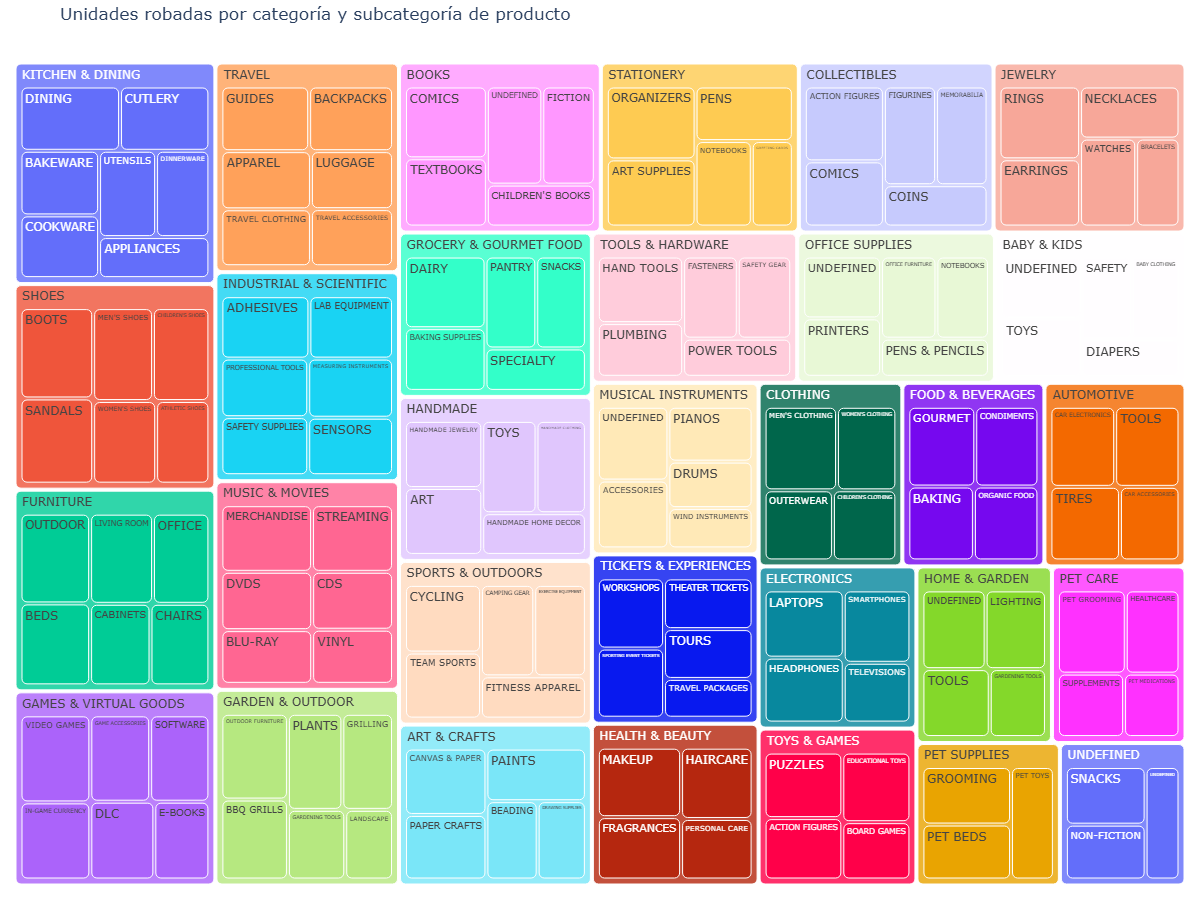
\includegraphics[width=0.8\textwidth]{imagenes/consultas_propias/treemap.png}
    \caption{Unidades de productos robados por categoría y subcategoría de producto.}
    \label{fig:robos_treemap}
\end{figure}

\begin{figure}[H]
    \centering
    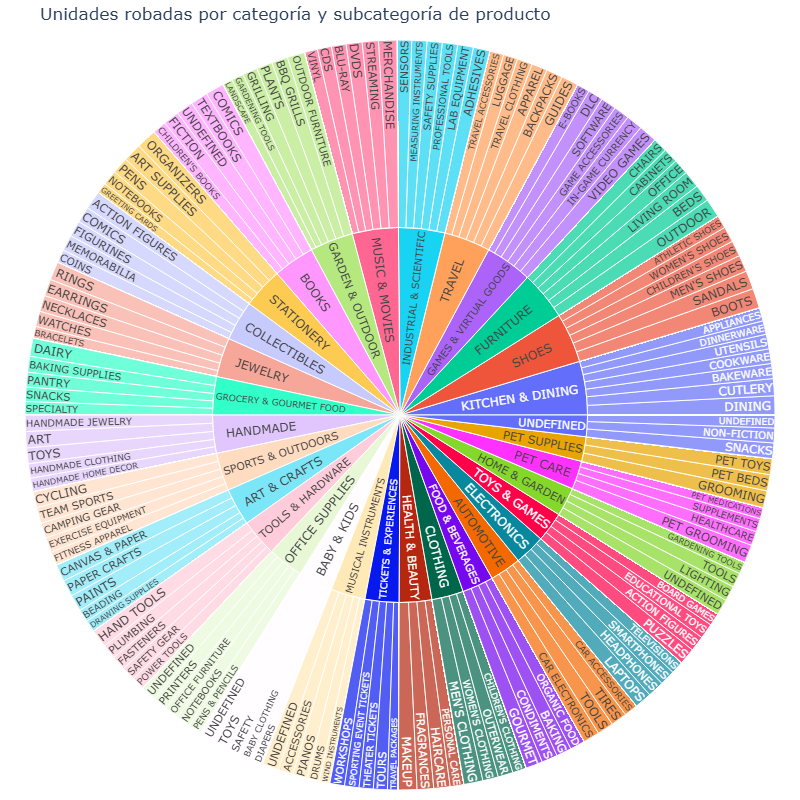
\includegraphics[width=0.6\textwidth]{imagenes/consultas_propias/sunburst.png}
    \caption{Unidades de productos robados por categoría y subcategoría de producto, visualizado como sunburst.}
    \label{fig:robos_sunburst}
\end{figure}


    \newpage
    \section{Anexo}
    \addtocontents{toc}{\protect\setcounter{tocdepth}{1}}
    \label{anexo}
\subsection{Output de la Consultas Propuestas por el Enunciado}
Estos outputs pueden encontrarse en el notebook \texttt{propuestas\_del\_enunciado.ipynb}. 
\subsubsection{Consulta 1}
\textbf{Output de la Validación}

\label{anexo:output_validacion_consulta1}
\begin{lstlisting}[style=console]
Filas totales en dataset orders: 4700000
Filas con estado no nulos: 4277862
Filas con estado nulo: 422138
Todas las filas que tienen estado nulo, tienen direccion de facturacion indefinida? Si
\end{lstlisting}

\textbf{Filtro de Estados}

\label{anexo:output_filtro_estados}
\begin{lstlisting}[language=Python]
not_states_filter = ~(
    orders["state"].str.contains("AA")   # Military Americas
    | orders["state"].str.contains("AE") # Military Europe
    | orders["state"].str.contains("AP") # Military Pacific
    | orders["state"].str.contains("FM") # Federated States of Micronesia
    | orders["state"].str.contains("MH") # Marshall Islands
    | orders["state"].str.contains("MP") # Northern Mariana Islands
    | orders["state"].str.contains("PW") # Palau
    | orders["state"].str.contains("GU") # Guam
    | orders["state"].str.contains("VI") # U.S. Virgin Islands
    | orders["state"].str.contains("AS") # American Samoa
    | orders["state"].str.contains("PR") # Puerto Rico
    | orders["state"].str.contains("DC") # District of Columbia
    | orders["state"].isna()             # Nulos
)
print("Cantidad de estados: ", orders.loc[not_states_filter]["state"].unique().size)
print("Estados considerados: ", orders.loc[not_states_filter]["state"].unique())
\end{lstlisting}
\begin{lstlisting}[style=console, aboveskip=0pt]
Cantidad de estados:  50
Estados considerados:  ['ND' 'NJ' 'MN' 'WI' 'OH' 'NV' 'MA' 'AZ' 'MO' 'VT' 'MI' 'NY' 'NM' 'PA'
 'WY' 'NE' 'WV' 'KY' 'WA' 'TX' 'OK' 'ME' 'KS' 'IN' 'FL' 'MD' 'MS' 'AL'
 'MT' 'ID' 'NC' 'AK' 'SD' 'NH' 'SC' 'CT' 'CA' 'CO' 'GA' 'IA' 'VA' 'OR'
 'DE' 'LA' 'UT' 'AR' 'IL' 'TN' 'RI' 'HI']
\end{lstlisting}

\textbf{Formateo de los Resultados}
El archivo json utilizado con los nombres de estado puede encontrarse junto con el código fuente del proyecto.
\label{anexo:output_formateo_resultados}
\begin{lstlisting}[language=Python, xleftmargin=70pt, xrightmargin=70pt]
import json
with open("state_names.json", "r") as f:
    state_names = json.load(f)

quantity_of_orders_with_discounts_by_state["Nombre del Estado"] = 
    quantity_of_orders_with_discounts_by_state["state"].map(state_names)

quantity_of_orders_with_discounts_by_state.rename(
    columns={
        "order_id": "Cantidad de Ordenes con Descuento",
        "state": "Codigo de Estado"
        }, inplace=True
    )
\end{lstlisting}

\subsubsection{Consulta 2}

\textbf{Códigos postales con 5 órdenes `Refunded'}

\label{anexo:output_codigos_postales_refunded}
\begin{lstlisting}[language=Python, xleftmargin=35pt, xrightmargin=35pt]
print("\nCodigos postales con 5 ordenes 'Refunded':")
print(amount_refunded_orders_by_zipcode.loc[amount_refunded_orders_by_zipcode["count"] == 5])
\end{lstlisting}
\begin{lstlisting}[style=console, aboveskip=0pt, xleftmargin=145pt, xrightmargin=145pt]
Codigos postales con 5 ordenes 'Refunded':
   zip_code  count
1     65247      5
2     38151      5
3      9045      5
4     14396      5
5     73291      5
6     91623      5
\end{lstlisting}

\textbf{Otros nombres que aparecen en órdenes `Refunded'}

\label{anexo:nombres_mas_comunes}
\begin{lstlisting}[language=Python, xleftmargin=105pt, xrightmargin=105pt]
print("\nOtros nombres que aparecen una sola vez:")
print(most_common_names.loc[most_common_names == 1].head(7))
\end{lstlisting}
\begin{lstlisting}[style=console, aboveskip=0pt, xleftmargin=145pt, xrightmargin=145pt]
Otros nombres que aparecen una sola vez:
first_name
ROBERT     1
CYNTHIA    1
JAY        1
MARIA      1
KAREN      1
CARLA      1
WILLIAM    1
\end{lstlisting}

\subsubsection{Consulta 3}
\textbf{Gráficos Heatmap resultantes}
\label{anexo:consulta3_heatmap}

\begin{figure}[H]
    \centering
    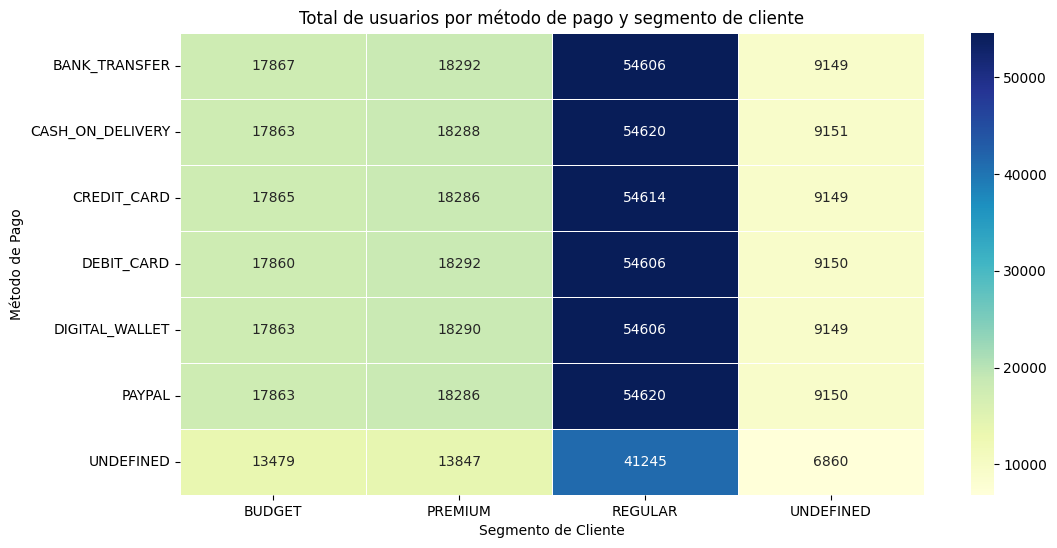
\includegraphics[width=0.8\textwidth]{imagenes/consulta3_heatmap1.png}
\end{figure}

\begin{figure}[H]
    \centering
    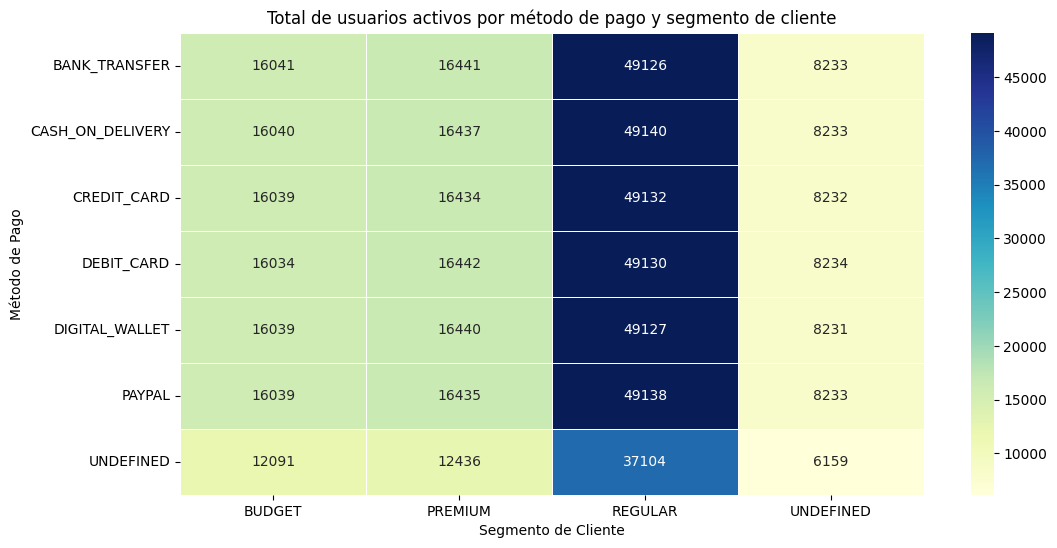
\includegraphics[width=0.8\textwidth]{imagenes/consulta3_heatmap2.png}
\end{figure}

\begin{figure}[H]
    \centering
    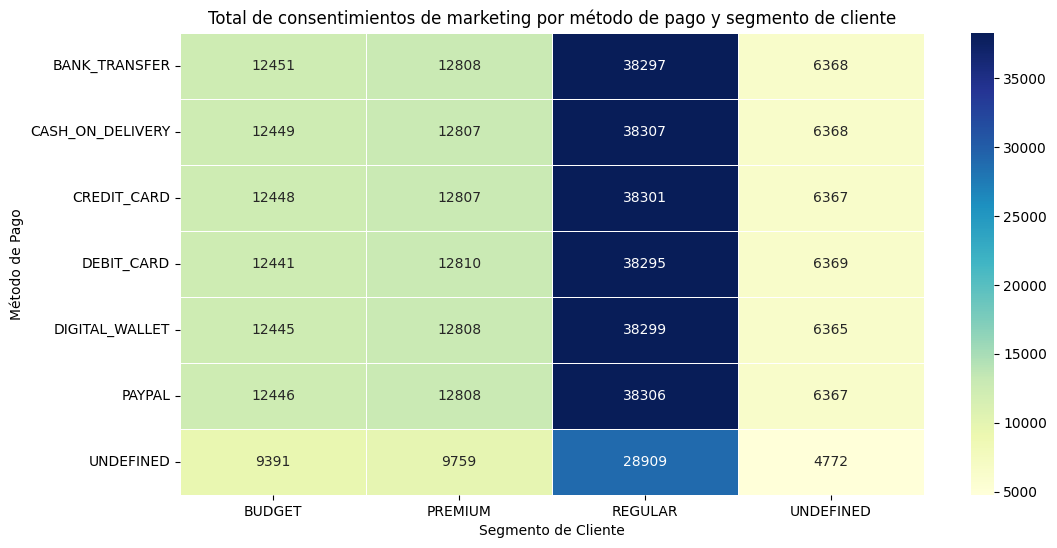
\includegraphics[width=0.8\textwidth]{imagenes/consulta3_heatmap3.png}
\end{figure}

\begin{figure}[H]
    \centering
    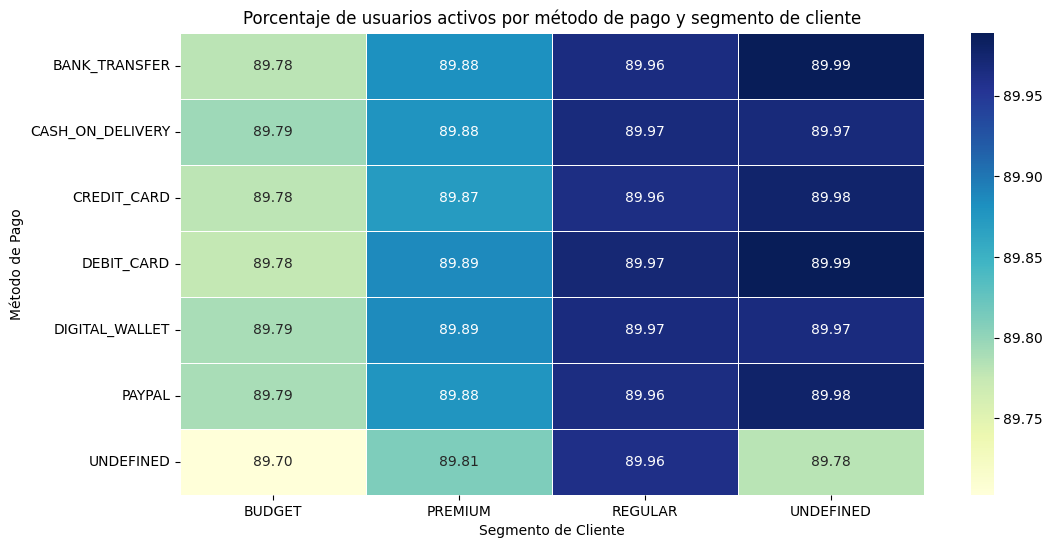
\includegraphics[width=0.8\textwidth]{imagenes/consulta3_heatmap4.png}
\end{figure}

\begin{figure}[H]
    \centering
    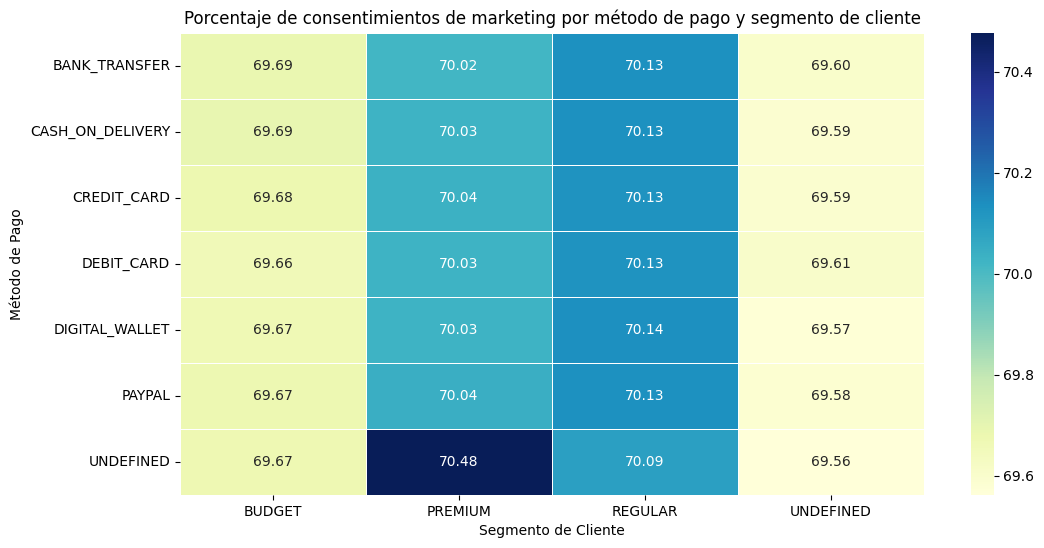
\includegraphics[width=0.8\textwidth]{imagenes/consulta3_heatmap5.png}
\end{figure}
    \addtocontents{toc}{\protect\setcounter{tocdepth}{2}}
    
\end{document}  